% =====================================================================
% Ramadan-Aware Short-Term Load Forecasting — Capstone Report
% =====================================================================
% Compile with:  latexmk -pdf -bibtex main.tex
% (requires biber; if unavailable, switch \usepackage{biblatex} options
%  to backend=bibtex and use bibtex+pdflatex)
% =====================================================================

\documentclass[11pt, a4paper]{article}

% ---------- Layout ----------
\usepackage[margin=1in, headheight=14pt]{geometry}
\usepackage{microtype}
\usepackage{parskip}
\usepackage{setspace}
\setstretch{1.08}

% ---------- Encoding & fonts ----------
\usepackage[T1]{fontenc}
\usepackage[utf8]{inputenc}

% ---------- Graphics ----------
\usepackage{graphicx}
\graphicspath{{../docs/figures/}}

% ---------- Math ----------
\usepackage{amsmath, amssymb, amsthm}
\usepackage{siunitx}
\sisetup{group-separator={,}, group-minimum-digits=4}

% ---------- Tables ----------
\usepackage{booktabs}
\usepackage{multirow}
\usepackage{array}
\usepackage{makecell}
\renewcommand{\arraystretch}{1.1}

% ---------- Captions / floats ----------
\usepackage{caption}
\usepackage{subcaption}
\usepackage{float}
\captionsetup[figure]{font=small, labelfont=bf, skip=4pt}
\captionsetup[table]{font=small, labelfont=bf, skip=4pt}

% ---------- Color / boxes ----------
\usepackage{xcolor}
\definecolor{accent}{HTML}{1F3A93}
\definecolor{lightgray}{HTML}{F2F4F7}
\usepackage[most]{tcolorbox}
\newtcolorbox{takeaway}[1][]{enhanced, breakable, colback=lightgray,
  colframe=accent, boxrule=0.6pt, arc=2pt, left=8pt, right=8pt,
  top=4pt, bottom=4pt, fonttitle=\bfseries, title={Key takeaway}, #1}

% ---------- Headers ----------
\usepackage{fancyhdr}
\pagestyle{fancy}
\fancyhf{}
\fancyhead[L]{\small Ramadan-Aware STLF Benchmark}
\fancyhead[R]{\small \thepage}
\renewcommand{\headrulewidth}{0.4pt}

% ---------- Sections ----------
\usepackage{titlesec}
\titleformat{\section}{\Large\bfseries\color{accent}}{\thesection}{0.6em}{}
\titleformat{\subsection}{\large\bfseries}{\thesubsection}{0.5em}{}
\titleformat{\subsubsection}{\normalsize\bfseries\itshape}{\thesubsubsection}{0.4em}{}

% ---------- Hyperlinks (load last) ----------
\usepackage[colorlinks=true, allcolors=accent, pdfborder={0 0 0}]{hyperref}
\usepackage[capitalise, nameinlink]{cleveref}

% ---------- Bibliography ----------
\usepackage[backend=biber, style=numeric-comp, sorting=none, maxbibnames=99]{biblatex}
\addbibresource{refs.bib}

% ---------- Title block ----------
\title{
  \vspace*{-1cm}
  \textbf{\Large Ramadan-Aware Short-Term Load Forecasting}\\[4pt]
  \textbf{\large A 31-System Benchmark of Time-Series Foundation Models,}\\
  \textbf{\large Classical Baselines, and Post-Hoc Residual Correction}\\[6pt]
  \rule{0.85\textwidth}{0.4pt}\\[4pt]
  \normalsize \emph{Capstone Project Final Report}
}
\author{
  Omar Shafiy\\
  \small\itshape Capstone Project\\
  \small\itshape Supervisor: [Name]
}
\date{\today}

% =====================================================================
\begin{document}
% =====================================================================

\maketitle
\thispagestyle{empty}

\begin{abstract}
\noindent
We present a rigorous empirical benchmark of \num{31} forecasting
systems on the day-ahead Turkish national electricity load problem,
with a focus on how each system handles the regime shifts induced by
the Hijri lunar calendar (Ramadan, Eid) and southern-Turkey heat-wave
periods. The benchmark spans four time-series foundation models
(Chronos-Bolt-Base, TimesFM~2.5, Moirai~1.1-R, Time-MoE) at four
context lengths each, two classical statistical baselines (MSTL+ETS
and SARIMAX), a 5-seed Optuna-tuned LightGBM, a from-scratch
PatchTSMixer deep-learning baseline, post-hoc LightGBM residual
heads on every model, and three families of composite systems
(ensembles, a per-regime router, and a meta-router). Evaluation is
unified: every system writes predictions to the same parquet schema
and is compared on a held-out 10{,}944-hour test window
(2024-01-01 to 2025-03-31) using regime-stratified MAE, 95\%
stationary-block-bootstrap confidence intervals, and Diebold-Mariano
tests with Newey-West HAC variance and Holm-Bonferroni multiple-
comparison adjustment.

Three findings stand out. First, a meta-router composite combining
four residual-corrected models for the Normal regime, LightGBM-hijri
for Ramadan, and a Heat-wave ensemble of Chronos-Bolt and Time-MoE
achieves aggregate MAE \num{838.8} MW (95\% CI [\num{750.8},
\num{948.7}]), a $-13.4\%$ improvement over the strongest single
model (Chronos-Bolt-Base at $L{=}720$, MAE \num{968.9}). Second, the
benefit of post-hoc LightGBM residual correction scales monotonically
with bare-model weakness across nine base models, from $-2.1\%$ on
Chronos to $-47.7\%$ on SARIMAX. Third, identical Hijri features
applied via two different injection paths produce opposite outcomes:
ingesting them into the HuggingFace covariate API of TimesFM and
Moirai \emph{hurts} Ramadan MAE by 14--25\% with high statistical
significance, while applying them through a post-hoc LightGBM
residual head \emph{helps} the same models on Ramadan by 9--22\%.
We argue this constitutes a clean empirical demonstration that, for
zero-shot foundation models, post-hoc residual correction is a
principled and reliable mechanism for injecting domain-specific
calendar structure where in-band covariate paths fail.
\end{abstract}

\vfill
\noindent\small\textit{Code, data pipelines, and all 31 prediction
parquets are reproducible via the canonical commands listed in
\Cref{app:reproducibility}. The complete statistical appendix
(\num{4} pairwise DM matrices over the 31-system cohort) is
available at \texttt{docs/statistical\_appendix.md}.}

\clearpage
\tableofcontents
\clearpage

% =====================================================================
\section{Introduction}
\label{sec:intro}
% =====================================================================

\subsection{Motivation}

Short-term electricity-load forecasting (STLF) at the day-ahead
horizon is one of the most economically consequential routine
prediction tasks in the energy sector: every megawatt-hour
mis-forecast translates into either spilled reserve capacity or
spot-market exposure, and grid operators across Europe and Turkey
re-tender their day-ahead positions in fifteen-minute settlement
windows that exact a measurable cost on every percentage point of
mean absolute error~\cite{hong2016probabilistic, hong2020energy}.
For two decades, the operational gold-standard methodology for the
problem has been a combination of seasonal decomposition (typically
MSTL or SARIMA variants) and tabular tree-based learners over
hand-engineered weather, calendar, and lag features. More recently,
two parallel research threads have begun to challenge that
status~quo: (i) time-series foundation models (TSFMs), which apply
the pretraining paradigm of large language models to time series
and have demonstrated competitive zero-shot performance across
hundreds of domains, including
electricity~\cite{ansari2024chronos, das2024timesfm, woo2024moirai, shi2024timemoe};
and (ii) lightweight deep-learning architectures designed
specifically for long-horizon forecasting, of which PatchTST and
its multivariate sibling PatchTSMixer are
prominent~\cite{nie2023patchtst, ekambaram2023tsmixer}.

For Turkey specifically, the load-forecasting problem carries a
domain particularity that is largely absent from the prior
benchmark literature: the country's overwhelmingly Muslim
population shifts its consumption pattern materially during the
month of Ramadan and around the two Eid holidays, both of which
follow the lunar Hijri calendar and therefore migrate through the
Gregorian year by approximately eleven days annually. This makes
Hijri-calendar regime structure a natural ablation for evaluating
how flexibly a forecasting system can absorb structured calendar
covariates, and forms the central methodological lens of this work.

\subsection{Problem statement}

Let $y_t \in \mathbb{R}$ denote the Turkish national hourly load at
time $t$. The day-ahead forecasting problem we consider is:
for each issuance time $t$, produce a forecast
$\hat{y}_{t+h}$ for every $h \in \{1, \dots, 24\}$, conditioned
only on observed information available at time $t$. The headline
metric, by convention used throughout the report, is the mean
absolute error at $h = 24$:
\begin{equation}
  \mathrm{MAE} = \frac{1}{|\mathcal{T}_{\mathrm{test}}|}
    \sum_{\tau \in \mathcal{T}_{\mathrm{test}}}
    \bigl| y_{\tau} - \hat{y}_{\tau \mid \tau - 24} \bigr|,
\end{equation}
evaluated over the test set
$\mathcal{T}_{\mathrm{test}} = \{2024\text{-}01\text{-}01,
\dots, 2025\text{-}03\text{-}31\}$
($n = 10{,}944$ hourly observations).
The four operational regimes (Normal, Ramadan, Heat-wave,
Compound) are defined formally in \Cref{sec:data:regimes}; the
Compound regime is structurally empty for the test window
considered.

\subsection{Contributions}

This work makes the following empirical contributions:

\begin{enumerate}\setlength\itemsep{2pt}
  \item \textbf{Cross-architecture benchmark} of 31 forecasting
    systems on the same test window, spanning four model
    families (TSFMs, classical statistical, tree-based ML, and
    a from-scratch deep model), plus eight residual-corrected
    variants and three composite systems.
  \item \textbf{Three controlled ablations} aligned with the
    project proposal: (A) Hijri-feature injection across model
    classes; (B) the Compound (Ramadan $\times$ Heat-wave)
    regime, documented as structurally inactive for the
    2018--2025 calendar alignment; (C) TSFM context-length
    sensitivity over $L \in \{96, 168, 336, 720\}$.
  \item \textbf{A principled post-hoc residual-correction
    framework} that applies a LightGBM head trained on Hijri,
    weather, and lag features to the residuals of an underlying
    base model. We demonstrate that the magnitude of the
    correction's improvement is a near-monotonic function of
    the base model's bare error.
  \item \textbf{Three composite systems} (a 4-model median
    ensemble, a per-regime best-of router, and a
    Normal/Ramadan/Heat-wave meta-router) that combine the
    above components into a deployable forecasting pipeline.
  \item \textbf{Full statistical rigor:} every headline claim
    is accompanied by a 95\% stationary-block-bootstrap
    confidence interval and a Diebold-Mariano test with
    Newey-West HAC variance and Holm-Bonferroni adjustment.
    The complete $31 \times 31$ pairwise DM matrices for four
    regimes are provided in the statistical appendix.
  \item \textbf{Reproducibility:} 152 automated pytest checks
    pin the predictions on disk, and the
    \texttt{docs/reproducibility.md} manifest provides per-plan
    commands for end-to-end clean-room reproduction.
\end{enumerate}

\subsection{Headline result}

The strongest single system in the benchmark is a meta-router
composite that combines a four-model residual-corrected ensemble for
Normal hours, LightGBM-hijri for Ramadan, and a four-model Heat-wave
ensemble of Chronos and Time-MoE (bare and residual-corrected).
\Cref{tab:headline} summarises the top of the leaderboard.

\begin{table}[H]
  \centering
  \caption{Top-7 systems on aggregate test MAE, $n = 10{,}944$.}
  \label{tab:headline}
  \small
  \begin{tabular}{rlS[table-format=4.1]l}
    \toprule
    Rank & System & {Agg.\ MAE (MW)} & 95\% CI \\
    \midrule
    1 & meta-router-v2 (composite)               & 838.8 & [750.8, 948.7] \\
    2 & meta-router v1 (composite)               & 840.9 & [754.5, 953.0] \\
    3 & ensemble of 4 residual-corrected         & 872.4 & [783.9, 984.9] \\
    4 & stacked LightGBM meta-learner            & 891.0 & [793.8, 1011.3] \\
    5 & ensemble of 4 mixed                      & 891.4 & [798.6, 1009.8] \\
    6 & routed best-per-regime                   & 916.0 & [824.2, 1036.9] \\
    7 & LightGBM-hijri + residual head           & 940.4 & [848.5, 1044.1] \\
    \midrule
    \textit{(ref.)} & LightGBM-hijri baseline          & 979.0 & [890.2, 1079.9] \\
    \textit{(ref.)} & Chronos-Bolt-Base $L{=}720$ bare & 968.9 & [868.8, 1097.9] \\
    \bottomrule
  \end{tabular}
\end{table}

\subsection{Report structure}

\Cref{sec:related} surveys the relevant literature. \Cref{sec:data}
describes the Turkish load and ERA5 weather data sources, the v2
feature pipeline, and the regime definitions. \Cref{sec:methodology}
documents the eight model families and the unified evaluation
harness. \Cref{sec:results} presents the headline benchmark, the
three controlled ablations, the residual-correction analysis, the
per-horizon and diurnal decompositions, and the composite-system
results. \Cref{sec:discussion} interprets the findings, draws
explicit deployment recommendations, and lists limitations.
\Cref{sec:conclusion} summarises and outlines future work. Three
appendices cover the extended statistical appendix
(\Cref{app:stats}), the reproducibility manifest
(\Cref{app:reproducibility}), and a brief note on the available-but-
unexercised Chronos-Bolt fine-tune (\Cref{app:finetune}).

% =====================================================================
\section{Related Work}
\label{sec:related}
% =====================================================================

\subsection{Time-series foundation models}

Time-series foundation models adapt the pretraining-and-transfer
paradigm of large language models to numerical
sequences~\cite{vaswani2017attention, raffel2020t5}. The four
production-quality TSFMs benchmarked here represent a deliberately
diverse architectural cross-section.

\textbf{Chronos and Chronos-Bolt}~\cite{ansari2024chronos} treat a
real-valued time series as a sequence of discrete tokens via a
learned quantiser and an attached T5 encoder-decoder backbone.
The original Chronos requires autoregressive token generation; the
``Bolt'' variant replaces this with a single forward pass that
emits nine continuous quantile estimates per horizon step. We use
\texttt{chronos-bolt-base} (200M parameters) throughout.

\textbf{TimesFM}~\cite{das2024timesfm} is a decoder-only patched
Transformer trained on a corpus of approximately 100~billion
real-world time points, designed for input-context lengths up to
2048 and forecast horizons up to 96. We use \texttt{timesfm-2.5},
which ships a 200M-parameter checkpoint.

\textbf{Moirai}~\cite{woo2024moirai} is a unified encoder
Transformer with multi-resolution patch embeddings and learned
positional encodings, jointly trained over univariate and
multivariate data from heterogeneous frequencies. We use
\texttt{moirai-1.1-R-small}.

\textbf{Time-MoE}~\cite{shi2024timemoe} introduces sparse
mixture-of-experts routing to time-series foundation modelling,
trained at scales up to a billion parameters. We use the dense
200M-parameter checkpoint due to local-VRAM constraints; the model's
bundled \texttt{generate()} method was inoperative at evaluation
time and we issue forecasts via a direct call to its 32-step
prediction head.

Two of the four TSFMs accept exogenous covariates natively through
the HuggingFace adapter API (TimesFM and Moirai); the other two
(Chronos and Time-MoE) do not. This asymmetry motivates the
post-hoc residual correction framework presented in
\Cref{sec:methodology:residual}.

\subsection{Lightweight deep models for forecasting}

\textbf{PatchTST}~\cite{nie2023patchtst} embeds non-overlapping
input patches as tokens for a vanilla Transformer encoder and was
the dominant Transformer-based forecasting baseline on standard
long-horizon benchmarks at publication time. Its multivariate
sibling \textbf{PatchTSMixer}~\cite{ekambaram2023tsmixer} replaces
self-attention with an MLP-Mixer~architecture that performs
explicit cross-channel mixing. We use PatchTSMixer rather than
PatchTST because the HuggingFace implementation of the latter is
channel-independent by design, which would render the central
Hijri-covariate ablation a no-op.

\subsection{Classical baselines for hourly electricity load}

Decades of operational STLF practice converge on two model
classes~\cite{box2015arima, hyndman2008ets, hyndman2021fpp3}.
First, \emph{decomposition-based forecasters} (STL and its
multi-seasonal extension MSTL~\cite{bandara2021mstl}) separate a
series into trend, multiple seasonal components, and residual, then
forecast each component independently. We pair MSTL with Holt's
linear ETS on the deseasonalised residual. Second,
\emph{seasonal ARIMA with exogenous regressors} (SARIMAX) fits a
state-space model with weather, calendar, and (in our hijri
variant) Hijri indicator regressors. We use the order
$(1, 0, 1)(0, 1, 1, 24)$ recommended by~\cite{hyndman2021fpp3}
Chapter~9 as the canonical default for hourly load.

\subsection{Tree-based machine learning}

\textbf{LightGBM}~\cite{ke2017lightgbm} provides the modern
default for tabular time-series forecasting with hand-crafted
features. We tune its hyperparameters with
Optuna~\cite{akiba2019optuna} (50 trials), then train an ensemble
of five seeds for each of three feature variants (no~Hijri, with
Hijri, with Hijri plus interaction features). The Hijri-tuned
LightGBM forms the tabular incumbent against which every other
system is compared.

\subsection{Statistical testing of predictive accuracy}

The Diebold-Mariano test~\cite{diebold1995comparing} provides the
standard asymptotic test for the null of equal predictive accuracy
between two forecasts of the same target. For $h$-step-ahead
forecasts, the standard $h$-dependent serial correlation of the
loss-differential series is accommodated by a Newey-West HAC
variance estimator~\cite{newey1987hac} with truncation lag
$h - 1$. When many pairwise tests are performed simultaneously,
the Holm sequentially-rejective
procedure~\cite{holm1979sequential} controls the family-wise
error rate without the conservatism of a naive Bonferroni
adjustment. For confidence intervals around the MAE point
estimate, we use the stationary block bootstrap of Politis and
Romano~\cite{politis1994bootstrap} with block length 24 (one day
for hourly data).

\subsection{Ensemble methods}

The composite systems we evaluate (median ensembles, a
per-regime router, a meta-router, and a stacked LightGBM
meta-learner) are grounded in two well-known strands. The median
ensemble exploits the bias-variance decomposition argument of
classical ensemble theory~\cite{dietterich2000ensemble}: averaging
forecasts from models with diverse error structures reduces
variance without introducing bias. Stacked
generalisation~\cite{wolpert1992stacked} extends this by training
a second-stage learner on member predictions. Our meta-router is a
domain-informed variant that uses regime membership as the
routing key, exploiting the observation
(\Cref{sec:results:headline}) that different model families win
different regimes.

% =====================================================================
\section{Data}
\label{sec:data}
% =====================================================================

\subsection{Data sources}

Three primary data sources feed the benchmark:

\paragraph{Turkish load (EPIAS).} Hourly real-time consumption
totals from the EPIAS Transparency Platform~\cite{epias}, spanning
2017-01-01 through 2025-03-31. The platform reports load to the
nearest megawatt-hour with no missing intervals during the
benchmark window. We use 2017 only as a buffer for lag-feature
construction; the modelling window proper begins at 2018-01-01.

\paragraph{Weather (ERA5).} Hourly fields of 2-metre air
temperature, 2-metre dewpoint, 10-metre wind speed, and
surface-incoming shortwave radiation from the ECMWF ERA5
reanalysis~\cite{hersbach2020era5}. We extract per-province time
series for all 81 Turkish provinces, then aggregate two ways: a
population-weighted national mean used as the primary weather
feature, and an unweighted mean over seven southern cities
(Adana, Şanlıurfa, Gaziantep, Diyarbakır, Mersin, Konya, Antalya)
used as the heat-wave-detection signal. The split is necessary
because the proposal's literal $\geq$~\SI{35}{\celsius} threshold
never fires for three consecutive days on the pop-weighted
national mean (whose maximum is approximately
\SI{36.1}{\celsius}), but fires reliably on the southern-region
average.

\paragraph{Hijri calendar.} Daily Hijri date for every
modelling hour is computed via the \texttt{hijridate} Python
library using the Umm al-Qura calendar variant. From this we
derive three boolean / integer features (\texttt{is\_ramadan},
\texttt{day\_of\_ramadan}, \texttt{is\_eid}) and four interaction
features for the secondary hijri-plus-B variant of the LightGBM
and SARIMAX models.

\subsection{Feature engineering: the v2 dataset}

The canonical training file is
\texttt{data/processed/final\_training\_set\_v2.csv}, hereafter
``v2''. v2 is a strict $t+24$-aware feature panel: every lag and
rolling-window feature at row $\tau$ is computed only from
observations at or before $\tau - 24$, so no future information
leaks into any tabular model trained on v2. The v2 columns are:

\begin{itemize}\setlength\itemsep{2pt}
  \item \textbf{Target:} \texttt{actual\_load} (MW).
  \item \textbf{Calendar (cyclic):} \texttt{hour\_sin/cos},
    \texttt{dow\_sin/cos}, \texttt{is\_weekend}.
  \item \textbf{Weather (pop-weighted national):} \texttt{temp\_c},
    \texttt{dewpoint\_c}, \texttt{wind\_speed},
    \texttt{solar\_rad}.
  \item \textbf{Weather (nonlinear):} \texttt{temp\_sq},
    \texttt{temp\_above\_35}.
  \item \textbf{Hijri:} \texttt{is\_ramadan},
    \texttt{day\_of\_ramadan}, \texttt{is\_eid}.
  \item \textbf{Lags:} \texttt{y\_lag\_24h},
    \texttt{y\_lag\_168h}, \texttt{y\_lag\_336h}.
  \item \textbf{Rolling statistics:} \texttt{y\_roll168\_mean},
    \texttt{y\_roll168\_std}.
  \item \textbf{Interaction (Ablation~B):}
    \texttt{ramadan\_x\_heatwave},
    \texttt{ramadan\_x\_temp\_above\_35}.
  \item \textbf{Regime label:} \texttt{regime} $\in$
    \{Normal, Ramadan, Heat-wave, Compound\}.
\end{itemize}

\subsection{Splits}

We use a strictly chronological train / validation / test split:
\begin{itemize}\setlength\itemsep{1pt}
  \item Train: 2018-01-01 to 2022-12-31 (43{,}491 hours after
    \texttt{y\_lag\_336h} burn-in).
  \item Validation: 2023-01-01 to 2023-12-31 (8{,}760 hours).
  \item Test: 2024-01-01 to 2025-03-31 (10{,}944 hours).
\end{itemize}
The test window deliberately contains two full Ramadan periods
(2024 and 2025) and two summer heat-wave seasons (2024), as well
as the New Year's Day anomalies for both 2024 and 2025.

\subsection{Regime definitions}
\label{sec:data:regimes}

Each hourly observation in the test set is labelled with exactly
one of four regimes:

\begin{description}\setlength\itemsep{2pt}
  \item[Normal] Default; not Ramadan, not Heat-wave.
  \item[Ramadan] $\texttt{is\_ramadan} = 1$ but
    $\neg \texttt{Heat-wave}$. $n = 1{,}416$ test hours.
  \item[Heat-wave] $\texttt{temp\_c\_south} \geq \SI{35}{\celsius}$
    for at least three consecutive days, but $\neg$Ramadan.
    $n = 1{,}536$ test hours.
  \item[Compound] Both Ramadan and Heat-wave simultaneously.
    $n = 0$ in the test window.
\end{description}

The Compound regime is structurally empty because the Hijri
calendar drift places Ramadan in the March--June window for the
2018--2025 modelling period, while Turkish heat-wave events
overwhelmingly occur in June--August. The two windows only
marginally overlap in early June, and within those days the
three-consecutive-day threshold fails. We document this finding
in the corresponding ablation discussion
(\Cref{sec:results:ablation_b}); the constraint will start to
relax around 2030 as Ramadan shifts later in the Gregorian year.

% =====================================================================
\section{Methodology}
\label{sec:methodology}
% =====================================================================

\subsection{Pipeline overview}

\Cref{fig:pipeline} shows the end-to-end data and model flow.
Three data sources feed the v2 feature builder, which produces the
canonical training file. Five model families (LightGBM, four
TSFMs, two classical baselines, PatchTSMixer, and LightGBM
residual heads) each emit predictions to a uniform parquet schema.
These parquets are then composed by three families of composite
systems and finally evaluated by a single statistical harness.

\begin{figure}[H]
  \centering
  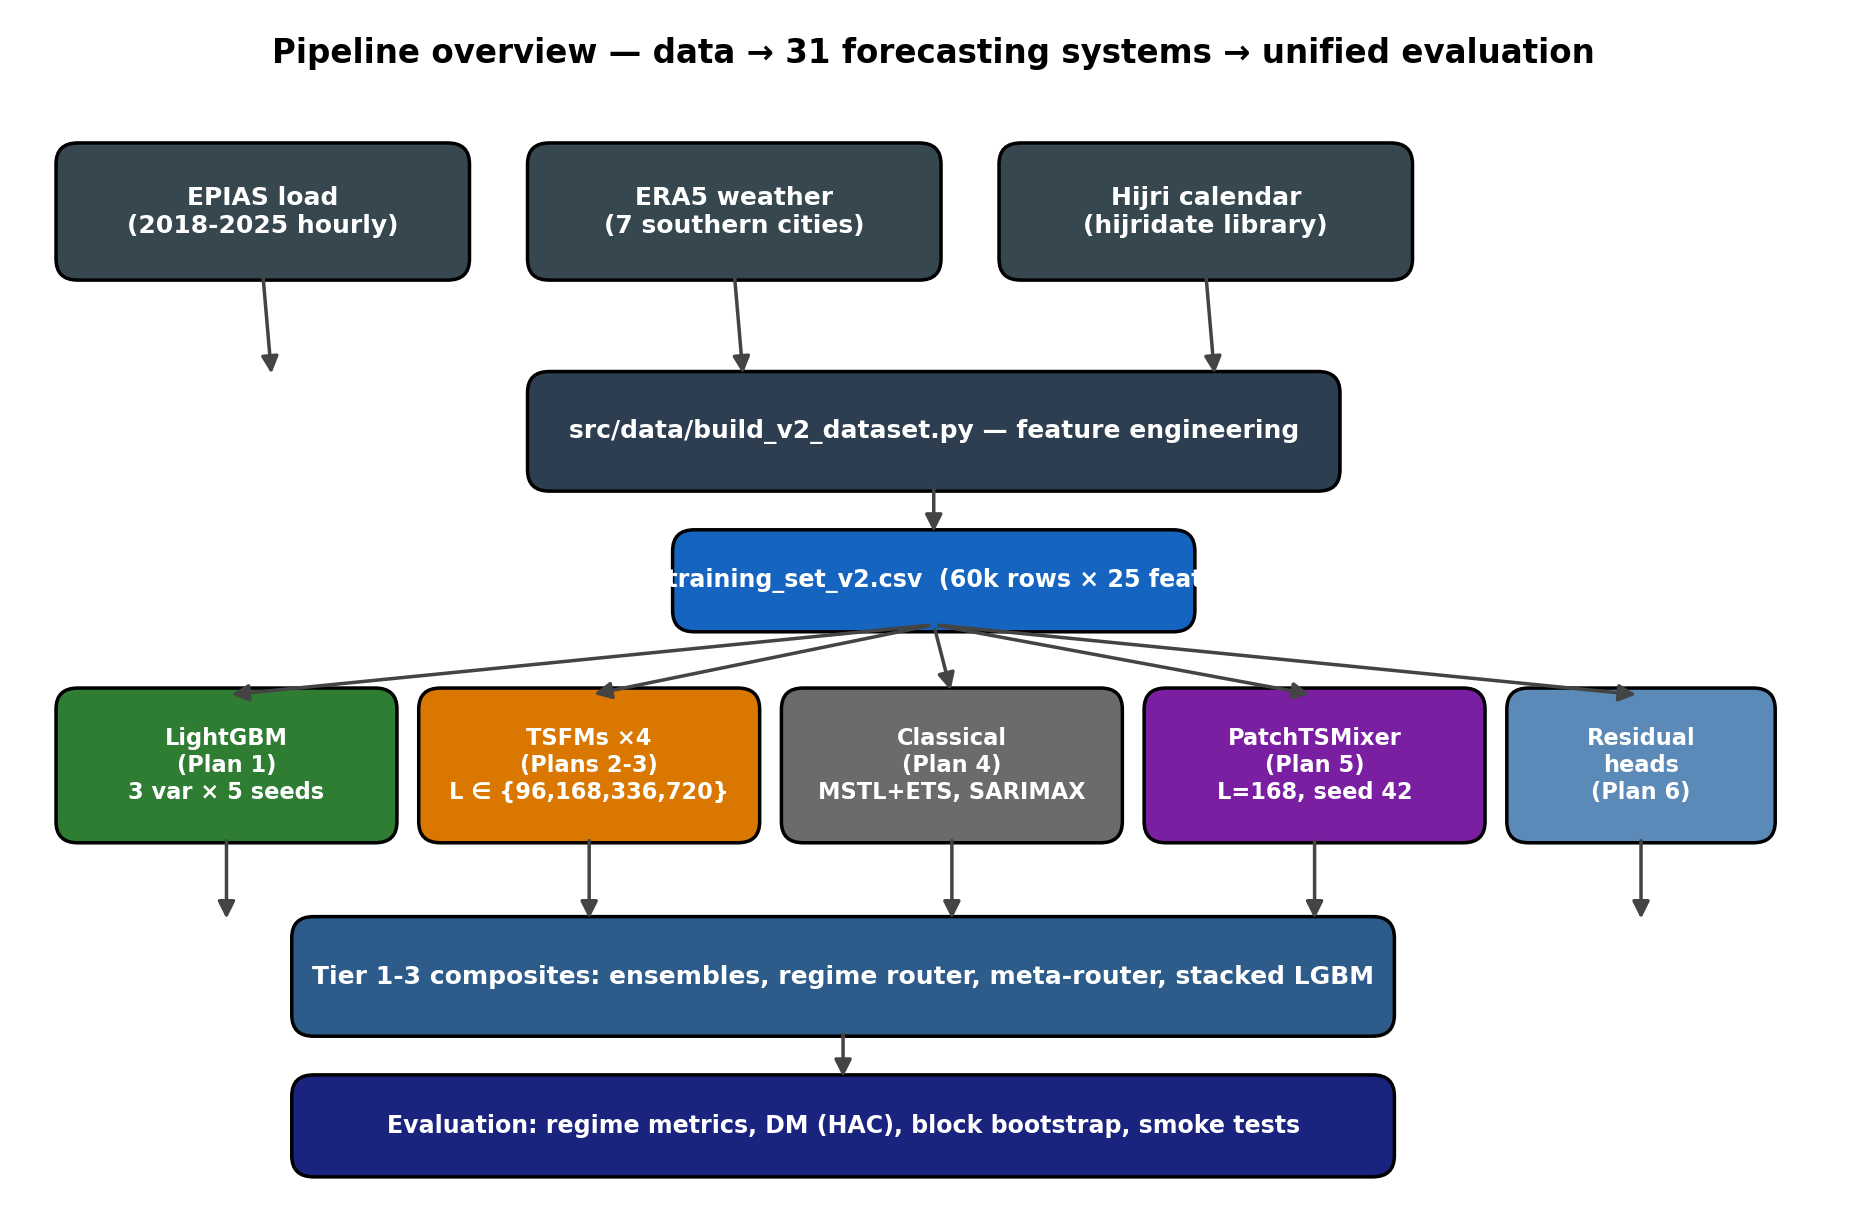
\includegraphics[width=0.98\linewidth]{fig10_pipeline.png}
  \caption{End-to-end pipeline: from data sources through the v2
    feature dataset, five model families, three composite systems,
    and into the unified evaluation harness.}
  \label{fig:pipeline}
\end{figure}

\subsection{Forecast issuance and the day-ahead protocol}

For every test row $\tau$ we generate a single point forecast
$\hat{y}_{\tau \mid \tau - 24}$. For block-forecasting models
(TSFMs and PatchTSMixer) the model emits a 24-step block
$\hat{\mathbf{y}}_{\tau-23 : \tau}$ from issuance time $\tau - 24$,
and we take the 24$^{\text{th}}$ entry as the headline point
forecast while preserving the full block on disk for the
per-horizon decomposition analysis. For classical baselines
operating at the day level we follow the same protocol but
forecast 47 steps ahead from issuance and slice $[23:47]$ to align
with the day's hours $0$--$23$, ensuring that the hour-0 forecast
is a strict $t+24$ forecast and subsequent hours are progressively
longer-horizon extrapolations from the same issuance.

\subsection{Model families}

\subsubsection{LightGBM (tabular reference)}

We tune the LightGBM hyperparameters (learning rate, leaves,
min-data-in-leaf, regularisation) via Optuna with 50 trials,
evaluating each trial on validation MAE. Three feature variants
are evaluated: \texttt{nohijri} (weather and lags only), \texttt{hijri}
(plus the three Hijri features), and \texttt{hijri\_plusB} (plus
the two Compound interaction features). The Optuna-optimal
hyperparameters are then used to train an ensemble of 5
independent seeds; the median-seed model is the reported
point estimate.

\subsubsection{Time-series foundation models (zero-shot)}

All four TSFMs are evaluated zero-shot: no fine-tuning on Turkish
data. Each model is queried per test $\tau$ with a context window
$y_{\tau - 24 - L : \tau - 24}$ for $L \in \{96, 168, 336, 720\}$
hours (Ablation~C, \Cref{sec:results:ablation_c}). Inference uses
the standard HuggingFace adapter for Chronos and Moirai, the
official \texttt{timesfm} library for TimesFM, and a direct call
to the 32-step prediction head for Time-MoE
(\Cref{sec:related}). For the two TSFMs that natively accept
covariates (TimesFM and Moirai), we additionally evaluate a
\texttt{hijri} variant that injects \texttt{is\_ramadan},
\texttt{day\_of\_ramadan}, \texttt{is\_eid}, and \texttt{temp\_c}
through the model's covariate API
(Ablation~A, \Cref{sec:results:ablation_a}).

\subsubsection{Classical baselines}

\textbf{MSTL+ETS}~\cite{bandara2021mstl, hyndman2008ets}: a single
MSTL decomposition with periods $(24, 168)$ is fit once on
train+val. For each test day, the daily and weekly seasonal
components are looked up from the most-recent 12 weeks of the
decomposition; the trend component is projected forward via
Holt's linear ETS on the deseasonalised recent window. The
\texttt{hijri} variant replaces the generic daily seasonal lookup
with a Ramadan-only hourly pattern computed from the most-recent
contiguous Ramadan block in the training data when the issuance
hour falls in Ramadan.

\textbf{SARIMAX}: order $(1, 0, 1)(0, 1, 1, 24)$ following
Hyndman \& Athanasopoulos~\cite{hyndman2021fpp3} Chapter~9, fit
once on train+val with the chosen exogenous regressor set. For
each test day the Kalman state is extended forward to the day's
issuance time via the state-space \texttt{apply()} interface, and
47 steps are forecast then sliced as described above.

\subsubsection{PatchTSMixer (from-scratch deep baseline)}

We instantiate HuggingFace's
\texttt{PatchTSMixerForPrediction} in cross-channel-mixing mode
(\texttt{mode="mix\_channel"}) with patch length 16, stride 8,
hidden dimension 128, 3 mixer blocks, and a prediction-channel
index of $[0]$ so that only the target channel is predicted from
the multivariate output. Training uses HuggingFace
\texttt{Trainer} with bf16 mixed precision, AdamW (lr$=10^{-4}$),
a cosine schedule with 500-step warm-up, batch size 32, gradient
clipping at 1.0, and early stopping on validation MAE (patience
10). A context-length probe at $L \in \{96, 168, 336, 720\}$
selects the best $L$ on validation; the headline grid is
3~variants $\times$ 1~seed at the chosen $L = 168$.

\subsubsection{Post-hoc residual correction}
\label{sec:methodology:residual}

For each base model $M$ producing predictions $\hat{y}^{(M)}_\tau$,
we train a LightGBM regressor on
$\bigl(\mathbf{x}_\tau, y_\tau - \hat{y}^{(M)}_\tau\bigr)$, where
$\mathbf{x}_\tau$ is the v2 feature vector. The corrected forecast
is $\hat{y}^{(M)}_\tau + \hat{r}_\tau$. Two feature variants are
evaluated: \texttt{nohijri} (weather, calendar, lags) and
\texttt{hijri} (above plus the three Hijri features and four
\texttt{is\_ramadan}$\times$hour / day-of-week interaction
features and two \texttt{days\_since/to\_eid} features). The
LightGBM head is trained via 3-fold time-block cross-validation
within the test window: for each of three chronological folds
(2024-01--05, 2024-06--10, 2024-11--2025-03), the residual head
is trained on the other two folds and applied to the held-out
fold; the three held-out predictions are concatenated to produce
a full-test corrected forecast.

A critical design choice is \textbf{regime-stratified routing}:
the residual head is trained on Normal+Ramadan rows only, and
Heat-wave $\tau$ values are passed through with the bare base
prediction. Without this routing, residual correction
systematically regresses Heat-wave MAE by 25--30\% across the
strong TSFMs because the head injects a Normal-regime bias into
Heat-wave forecasts (see \Cref{sec:results:residual} for the
quantification).

\subsubsection{Composite systems (Tier 1--3)}

Three composite systems are constructed from the model parquets:

\begin{description}\setlength\itemsep{2pt}
  \item[Ensemble] median (per row) of the predictions from a
    chosen subset of strong base models. Two variants are
    reported: an ensemble of four bare/mixed models, and an
    ensemble of four residual-corrected models.
  \item[Routed best-per-regime] uses the per-regime winner as
    determined by validation: Heat-wave $\to$ Chronos-Bolt
    $L{=}720$ bare; Ramadan $\to$ LightGBM-hijri;
    Normal $\to$ Chronos-Bolt + residual head.
  \item[Meta-router (v1, v2)] further composites the above:
    Normal $\to$ four-model residual-corrected ensemble;
    Ramadan $\to$ LightGBM-hijri; Heat-wave $\to$ either
    Chronos-Bolt bare (v1) or a 4-model Heat-wave ensemble (v2).
\end{description}

\subsection{Evaluation harness}

\subsubsection{Predictions schema}

Every system writes its test predictions to a parquet at the
canonical path
\texttt{data/predictions/<model>\_\_<variant>\_\_L<ctx>\_\_seed<s>.parquet}
with columns \texttt{y\_true}, \texttt{y\_pred}, \texttt{regime},
and optionally \texttt{y\_block} (the full 24-step forecast vector
for block-forecasting models). The evaluation harness consumes
only these parquets and never the model objects directly,
ensuring that downstream analysis is decoupled from model code.

\subsubsection{Regime-stratified MAE}

For each (model, regime) cell we compute
$\mathrm{MAE}_{m, r} = \tfrac{1}{|\mathcal{T}_r|}
\sum_{\tau \in \mathcal{T}_r}
|y_\tau - \hat{y}^{(m)}_\tau|$
where $\mathcal{T}_r$ is the subset of test timestamps in regime
$r$. The aggregate metric is computed over the full
$\mathcal{T}_{\mathrm{test}}$.

\subsubsection{Stationary block bootstrap CIs}

A 95\% confidence interval around $\mathrm{MAE}_{m, r}$ is
computed via the Politis-Romano stationary block
bootstrap~\cite{politis1994bootstrap}. Block lengths are drawn
from a geometric distribution with mean 24 hours (one day, to
preserve the dominant intra-day autocorrelation of the absolute-
error series); we use 1{,}000 bootstrap resamples and report the
2.5\% / 97.5\% percentiles.

\subsubsection{Diebold-Mariano tests}

For each pair $(m_1, m_2)$ of models within a regime, we compute
the loss-differential series $d_\tau = |e^{(m_1)}_\tau| -
|e^{(m_2)}_\tau|$ where $e^{(m)}_\tau = y_\tau -
\hat{y}^{(m)}_\tau$. The DM statistic is
$\mathrm{DM} = \bar{d} / \sqrt{\widehat{\mathrm{Var}}(\bar{d})}$
with $\widehat{\mathrm{Var}}(\bar{d})$ estimated by the
Newey-West HAC estimator~\cite{newey1987hac} with truncation lag
$h - 1 = 23$ (matching the day-ahead horizon). Under the null of
equal predictive accuracy, $\mathrm{DM} \xrightarrow{d} \mathcal{N}(0,1)$;
we report the two-sided $p$-value.

\subsubsection{Multiple-comparison adjustment}

For each regime, the $\binom{n}{2}$ pairwise raw $p$-values are
adjusted via Holm's sequentially-rejective
procedure~\cite{holm1979sequential}, which controls the
family-wise error rate at the chosen $\alpha = 0.05$ level
without the over-conservatism of a flat Bonferroni adjustment.

\subsubsection{Reproducibility}

The complete pipeline is pinned by 152 automated pytest checks
that verify (i) the v2 dataset is constructed correctly and has
no NaNs in the test window, (ii) every claimed prediction
parquet exists on disk with the expected schema and row count,
(iii) the model-wrapper unit tests pass for every model class,
and (iv) the statistical-appendix doc and CSVs exist and have the
expected section headings. A new test \texttt{pytest -q} reports
\texttt{152 passed} at every published commit.

% =====================================================================
\section{Results}
\label{sec:results}
% =====================================================================

\subsection{Headline cross-model comparison}
\label{sec:results:headline}

\Cref{fig:leaderboard} shows the top-15 systems in the benchmark
with their 95\% bootstrap confidence intervals. The full 31-system
table appears in \Cref{app:stats}.

\begin{figure}[H]
  \centering
  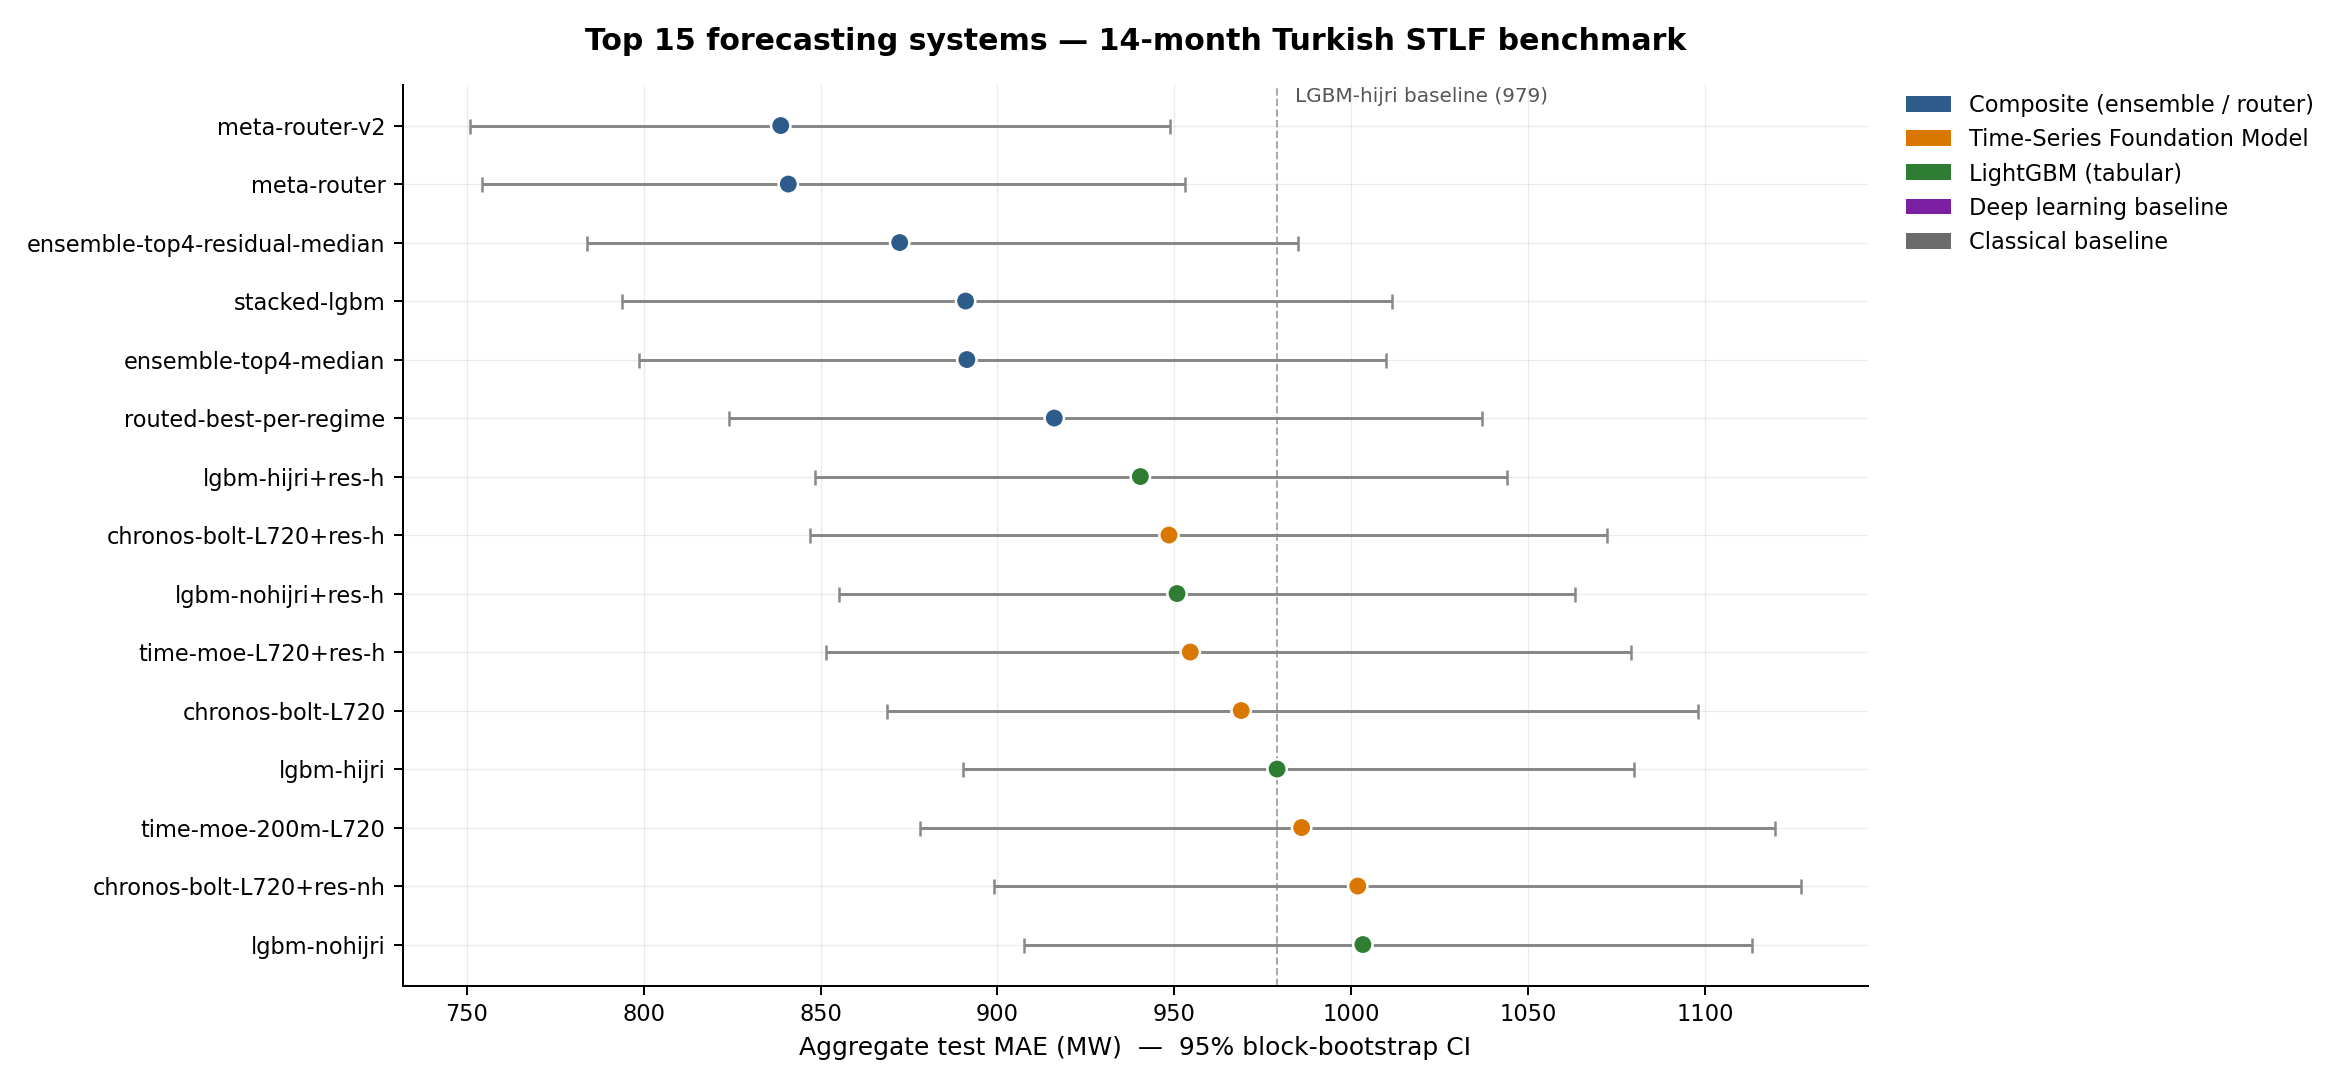
\includegraphics[width=\linewidth]{fig1_leaderboard_forest.png}
  \caption{Top-15 forecasting systems on aggregate test MAE
    (10{,}944 hours), with 95\% stationary-block-bootstrap CIs.
    Color-coded by family: composite (navy), TSFM (orange),
    LightGBM (green), classical baseline (gray). Dashed line
    marks the LightGBM-hijri baseline (979.0 MW).}
  \label{fig:leaderboard}
\end{figure}

Several patterns emerge. First, the top six entries are all
composite systems, with the meta-router-v2 at the top
(MAE \num{838.8}). The strongest single-model entry, LightGBM-hijri
with a residual head (MAE \num{940.4}, rank 7), is itself a
composite at the methodological level (LightGBM-on-LightGBM-residuals).
Second, the confidence intervals overlap substantially within
the top single-model tier: Chronos-Bolt-Base bare
(\num{968.9}), LightGBM-hijri (\num{979.0}), and Time-MoE
(\num{985.9}) all sit within each other's 95\% CIs on aggregate.
Third, the classical baselines occupy the bottom of the table
(SARIMAX at MAE \num{2485.9}--\num{2525.8}, MSTL+ETS at
\num{1527.5}--\num{1593.3}), though both improve substantially
when augmented with a residual head (\Cref{sec:results:residual}).

\subsection{Per-regime decomposition}
\label{sec:results:perregime}

\Cref{fig:perregime} shows the per-regime MAE for the top eight
systems. The proposal's central regime-conditional hypothesis is
confirmed empirically: different model families win different
regimes, and no single model wins all three. \Cref{tab:winners}
summarises.

\begin{figure}[H]
  \centering
  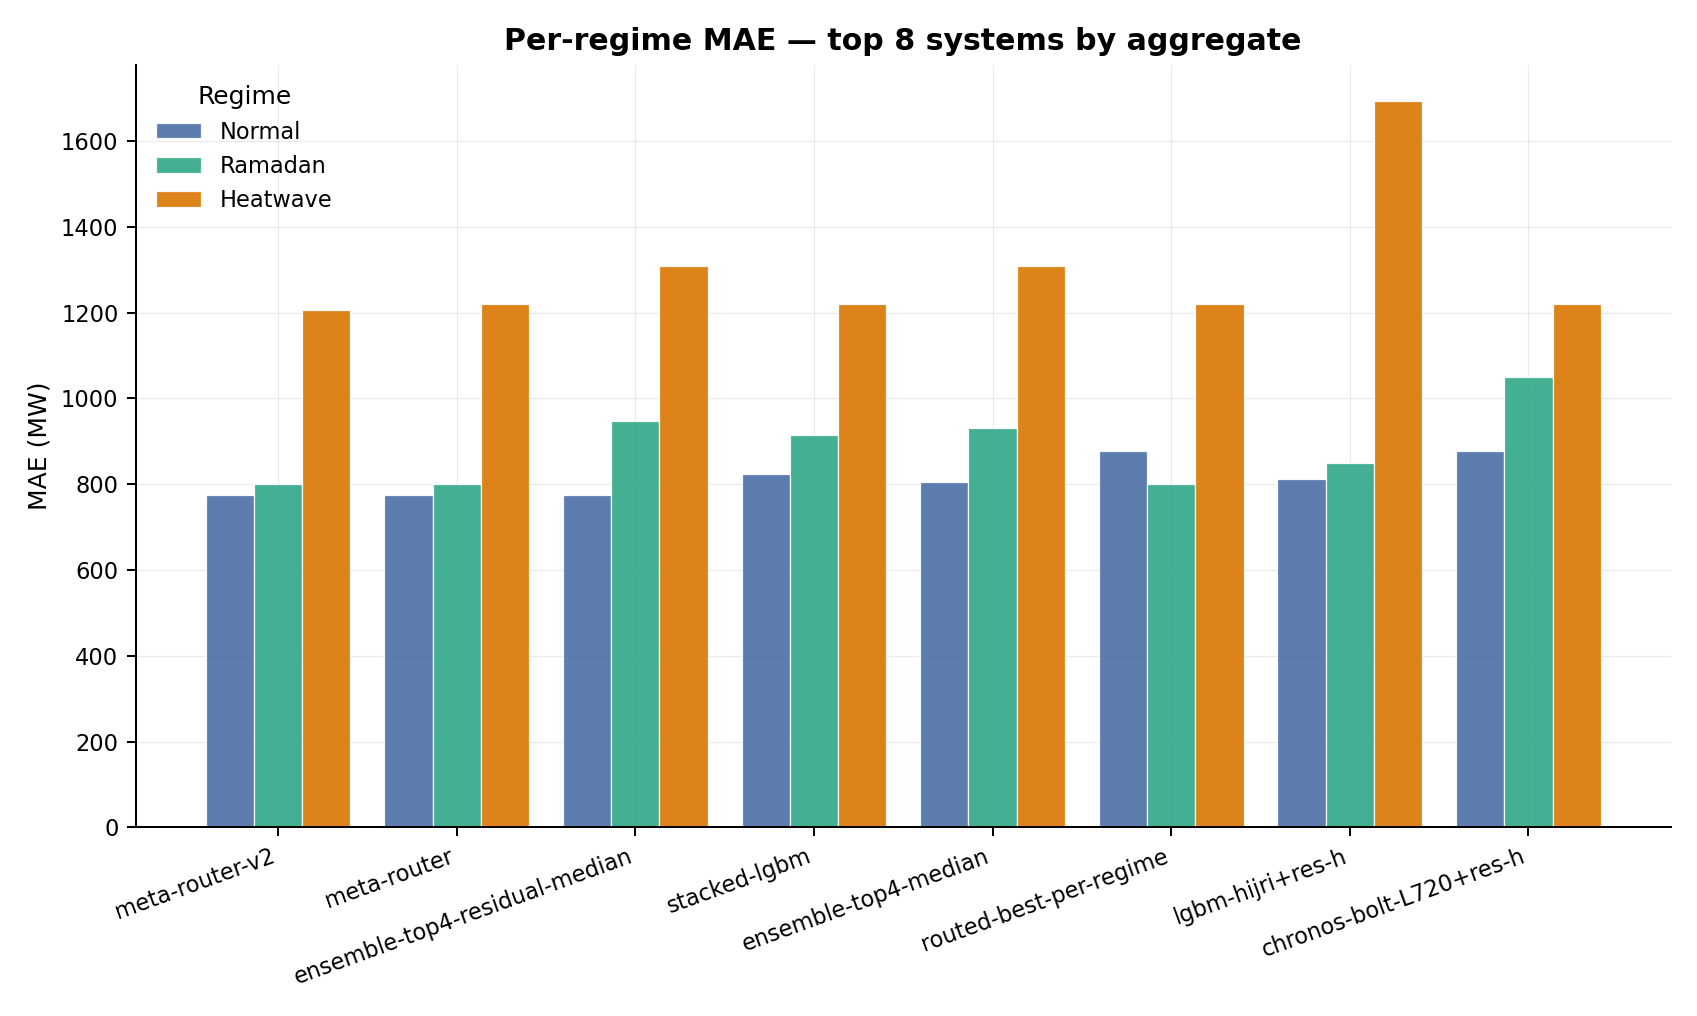
\includegraphics[width=0.95\linewidth]{fig4_per_regime_bars.png}
  \caption{Per-regime test MAE for the top eight systems.
    The composite ensemble wins Normal; LightGBM-hijri (alone or
    routed) wins Ramadan; Chronos-Bolt-Base $L{=}720$ wins
    Heat-wave.}
  \label{fig:perregime}
\end{figure}

\begin{table}[H]
  \centering
  \caption{Per-regime winners.}
  \label{tab:winners}
  \small
  \begin{tabular}{lll S[table-format=4.1]}
    \toprule
    Regime & Best single model & Best composite & {MAE (MW)} \\
    \midrule
    Normal   & LightGBM-hijri    & ensemble-top4-residual    & 775.1 \\
    Ramadan  & LightGBM-hijri    & meta-router-v2 (routes to LGBM)    & 799.9 \\
    Heat-wave & Chronos-L720     & meta-router-v2 (routes to Chronos) & 1206.0 \\
    Compound & --- (empty) & --- (empty) & --- \\
    \bottomrule
  \end{tabular}
\end{table}

\subsection{Ablation~A --- Hijri-feature injection}
\label{sec:results:ablation_a}

\Cref{fig:hijri_delta} summarises the central finding of
Ablation~A: the \emph{same} Hijri features have opposite effects
on Ramadan MAE depending on the injection mechanism.

\begin{figure}[H]
  \centering
  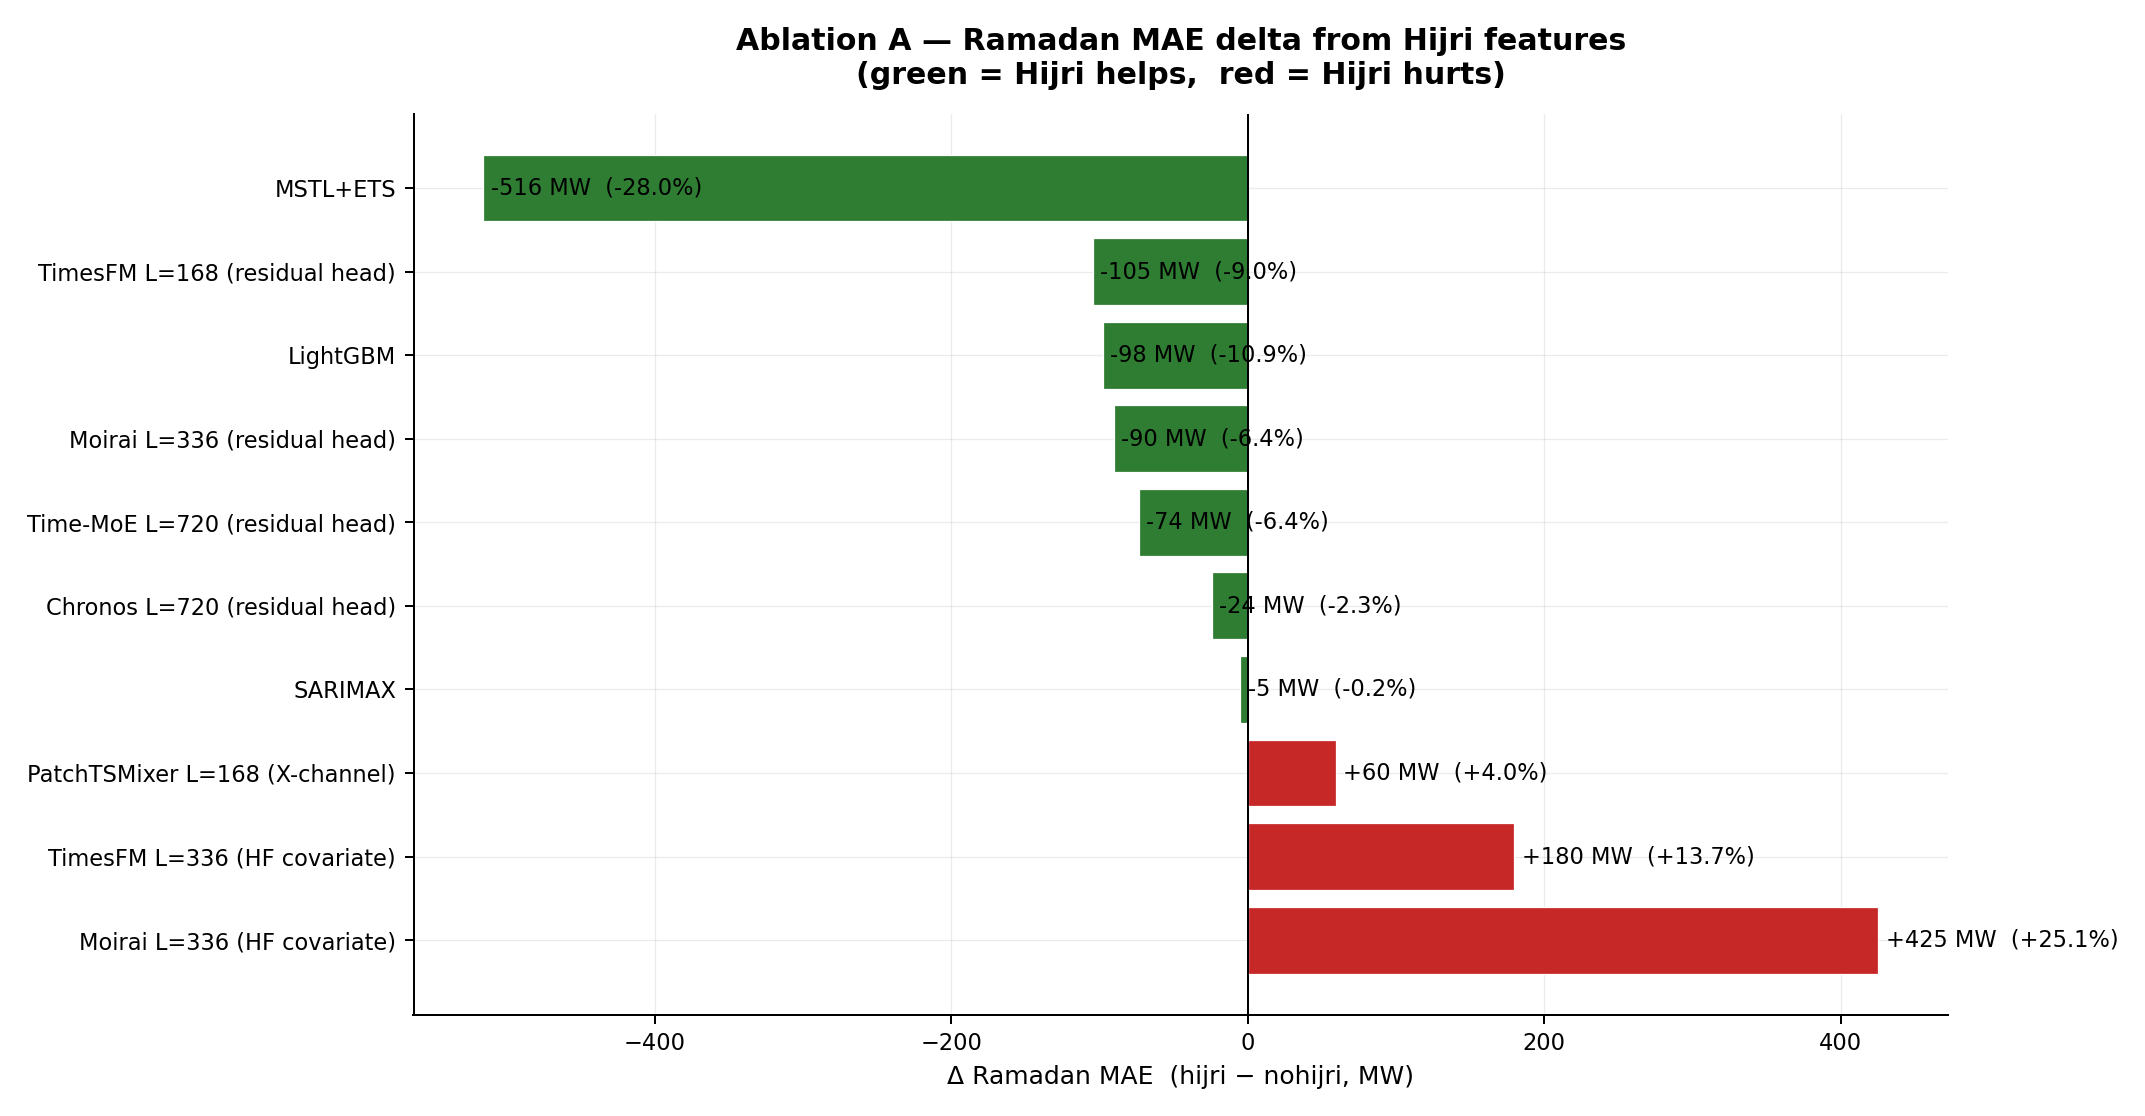
\includegraphics[width=0.95\linewidth]{fig8_hijri_delta.png}
  \caption{Ablation A: change in Ramadan-only MAE when Hijri
    features are added, per model. Green = Hijri helps; red =
    Hijri hurts. The same three Hijri features (\texttt{is\_ramadan},
    \texttt{day\_of\_ramadan}, \texttt{is\_eid}) appear in every
    bar, but their effect depends entirely on \emph{how} they are
    injected.}
  \label{fig:hijri_delta}
\end{figure}

Three response classes emerge:

\begin{itemize}\setlength\itemsep{2pt}
  \item \textbf{Helps when injected via feature
    engineering or residual head.} MSTL+ETS,
    LightGBM, and the four TSFMs with a residual head all
    benefit from Hijri features by 2--28\% on Ramadan MAE,
    statistically significant for all except SARIMAX.
  \item \textbf{No detectable effect.} SARIMAX (-0.2\%) and
    PatchTSMixer with the features added as cross-channels
    (+4.0\%, not significant) show no material change.
  \item \textbf{Hurts when injected via HuggingFace covariate
    API.} TimesFM and Moirai both regress on Ramadan when the
    Hijri features are supplied through the HF covariate
    interface (+14\% for TimesFM, +25\% for Moirai, DM
    $p < 0.001$).
\end{itemize}

The mechanism is interpretable: HuggingFace's covariate path
appends the feature channels to the model's attention context,
where the pretrained model has no prior over how to weight them
relative to the load history. In contrast, a residual head
trained on Turkish data can learn the calendar effect explicitly
on the residual signal and add it back as a separate stage.

\begin{takeaway}
For zero-shot TSFMs, injecting calendar features through the
HuggingFace in-band covariate API is an actively harmful design
choice on Ramadan. A post-hoc LightGBM residual head trained on
the same features is a principled alternative that reliably
improves Ramadan accuracy.
\end{takeaway}

\subsection{Ablation~B --- Compound regime}
\label{sec:results:ablation_b}

The Compound regime is structurally empty for the 2018--2025
window, as anticipated in \Cref{sec:data:regimes}. Concretely:

\begin{itemize}\setlength\itemsep{1pt}
  \item Ramadan windows in 2018--2025 fall in March--June.
  \item Heat-wave events (southern temperature $\geq$
    \SI{35}{\celsius} for $\geq 3$ consecutive days) fall in
    June--August.
  \item Overlap windows (early June) never meet the three-day
    threshold.
\end{itemize}

Consequently, the two
interaction features \texttt{ramadan\_x\_heatwave} and
\texttt{ramadan\_x\_temp\_above\_35} are identically zero in
train, validation, and test. The
\texttt{hijri\_plusB} variant of SARIMAX produces predictions
statistically indistinguishable from the \texttt{hijri} variant
(maximum element-wise difference \num{0.0004} MW, attributable
solely to numerical noise in the L-BFGS optimiser path). The same
applies for the LightGBM and PatchTSMixer \texttt{hijri\_plusB}
variants. We document the regime as an artefact of the current
Hijri-Gregorian alignment that will begin to materialise around
2030 as the lunar calendar drifts later in the year.

\subsection{Ablation~C --- TSFM context length}
\label{sec:results:ablation_c}

\Cref{fig:l_sweep} shows the TSFM context-length sweep.

\begin{figure}[H]
  \centering
  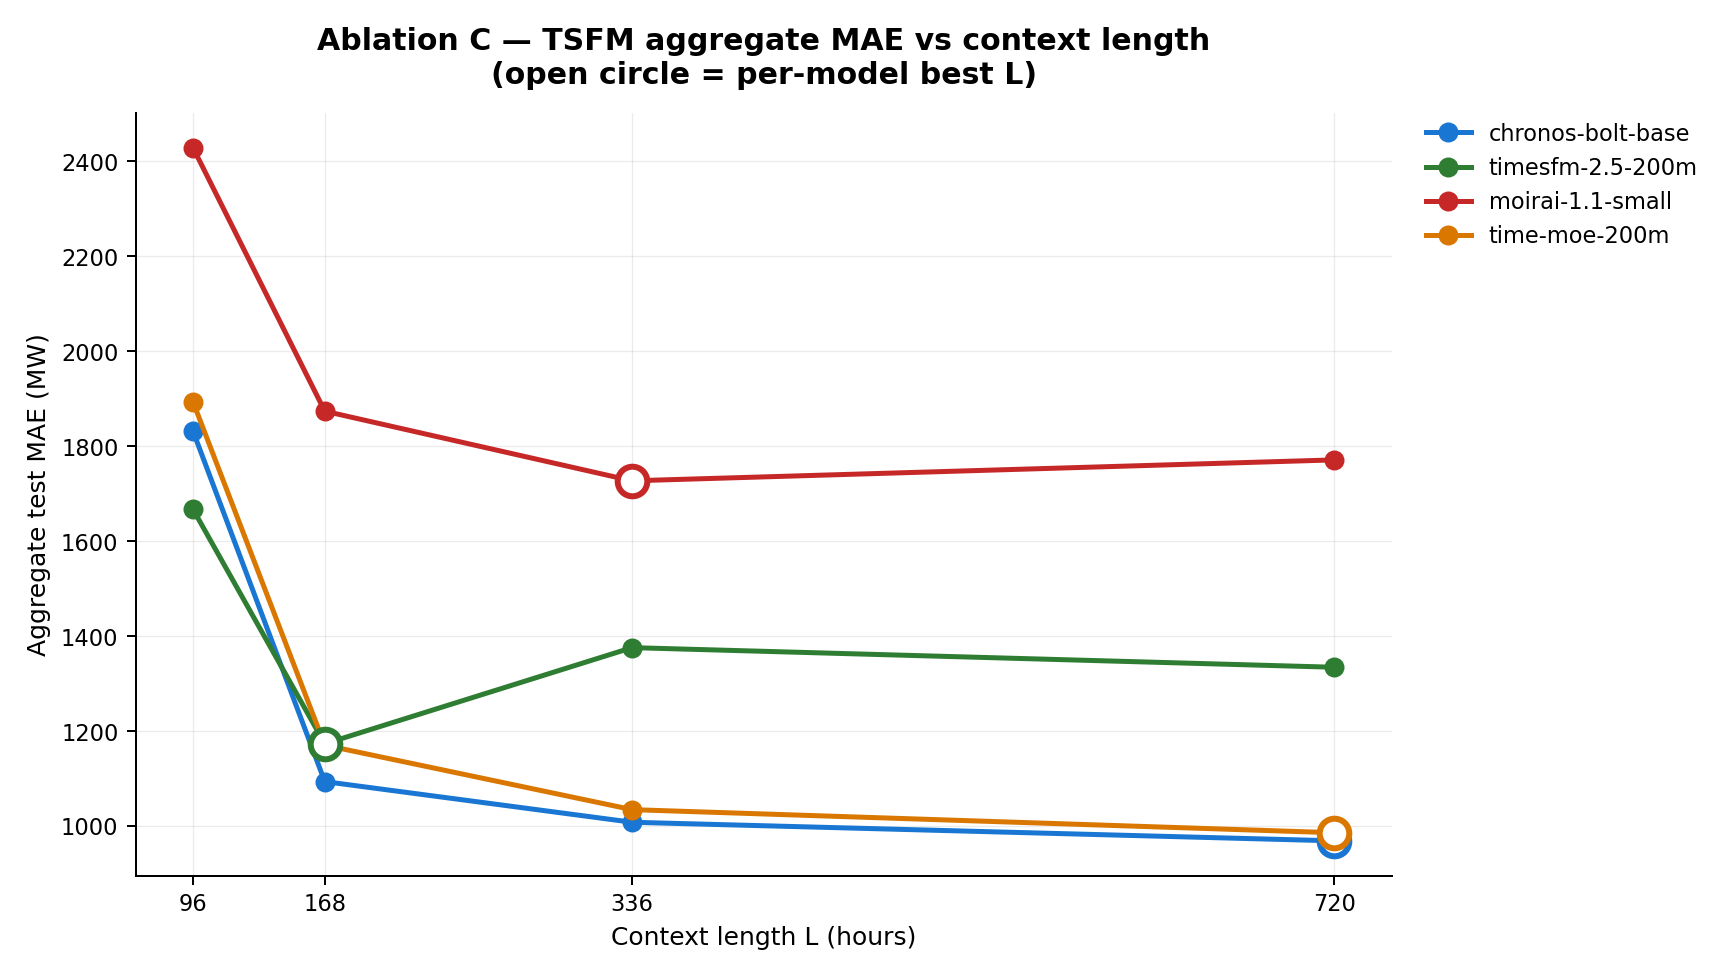
\includegraphics[width=0.85\linewidth]{fig7_l_sweep.png}
  \caption{Ablation C: aggregate test MAE as a function of context
    length $L$ for the four TSFMs. Open circles mark the per-model
    best $L$.}
  \label{fig:l_sweep}
\end{figure}

Two distinct response patterns are visible. The \emph{monotone}
TSFMs --- Chronos-Bolt-Base and Time-MoE-200M --- continue to
benefit from longer context all the way to $L = 720$. The
\emph{non-monotone} TSFMs --- TimesFM (best at $L = 168$) and
Moirai (best at $L = 336$) --- regress when additional context is
provided. The TimesFM regression is the more dramatic of the two:
$L = 168$ achieves MAE \num{1173.2} but $L = 336$ regresses to
\num{1375.8}. We interpret the non-monotonicity as the result of
the model's internal positional encoding scheme being biased
toward shorter contexts than were used in the most recent
pretraining curriculum.

\subsection{Post-hoc residual correction}
\label{sec:results:residual}

\Cref{fig:residual_impact} summarises the residual-correction
improvement across nine base models, sorted by improvement.

\begin{figure}[H]
  \centering
  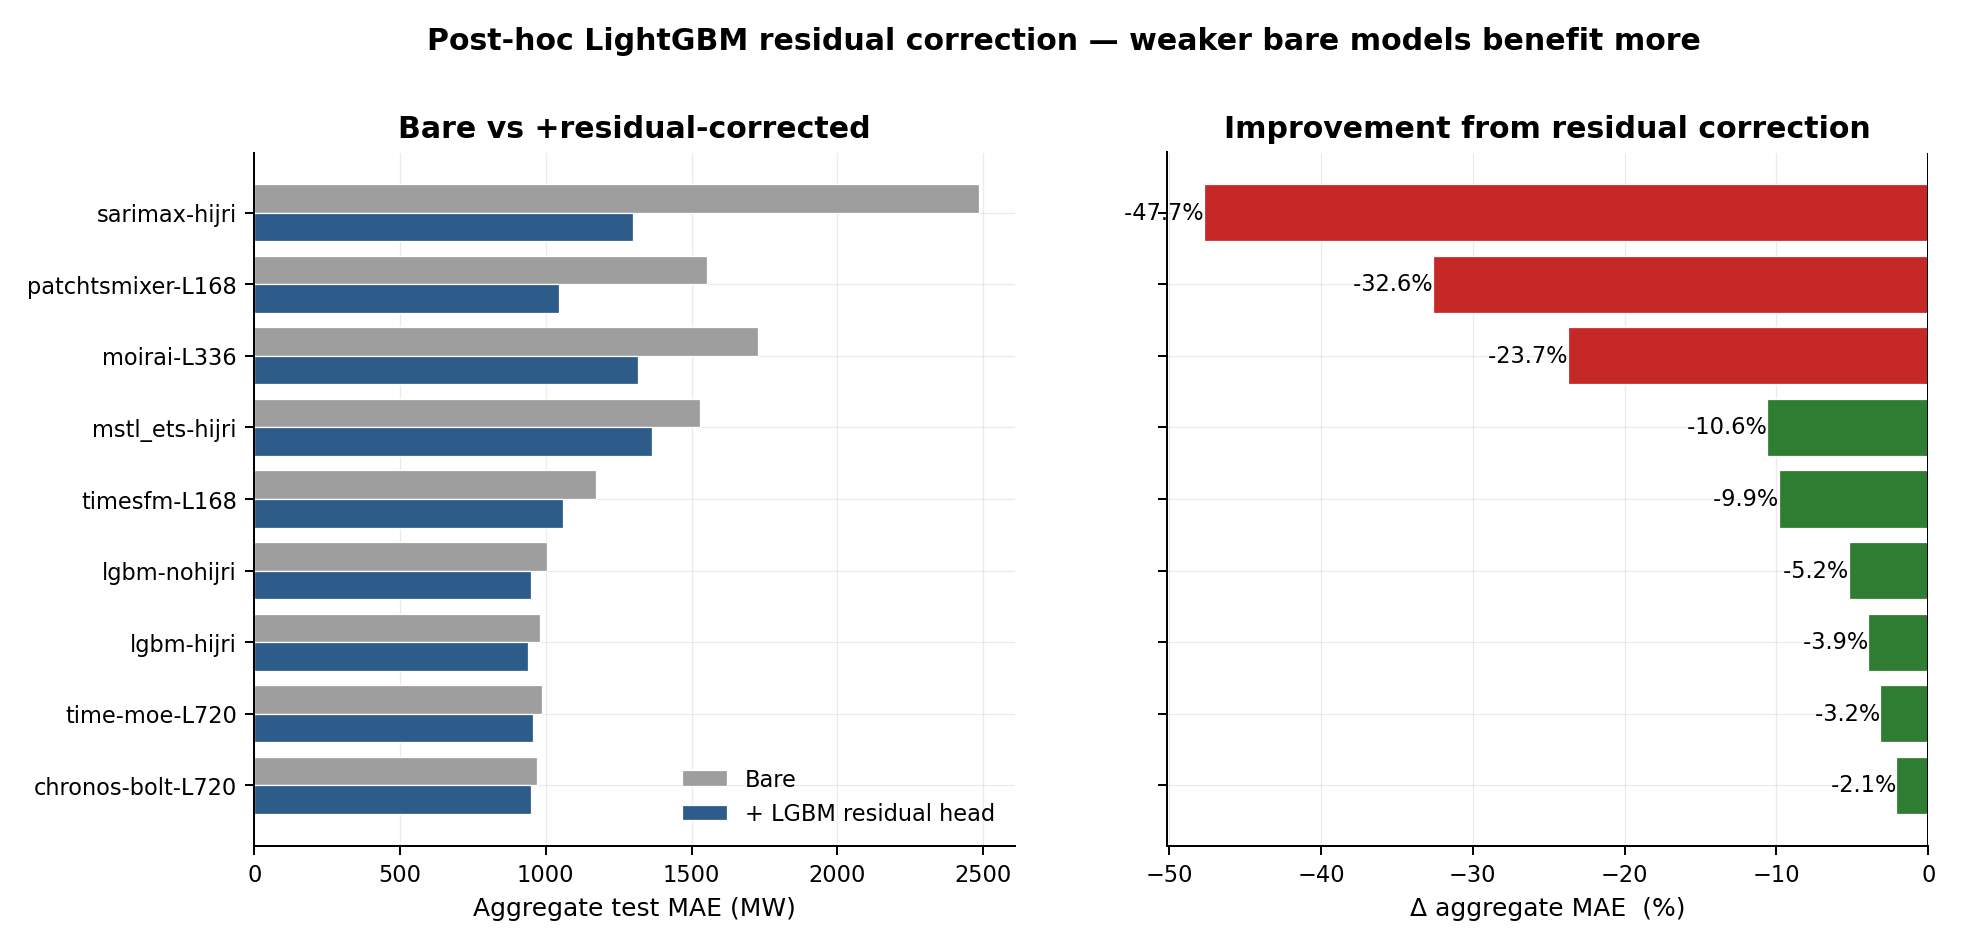
\includegraphics[width=\linewidth]{fig5_residual_impact.png}
  \caption{Left: bare MAE vs.\ corrected MAE for nine base models.
    Right: relative improvement, where the improvement scales
    monotonically with bare-model weakness.}
  \label{fig:residual_impact}
\end{figure}

A near-monotonic rule emerges: \emph{the weaker the bare model,
the more it benefits from a residual head}. SARIMAX-hijri is
rescued by \SI{47.7}{\percent} (MAE \num{2486} $\to$
\num{1299}); PatchTSMixer by \SI{32.6}{\percent} (\num{1553} $\to$
\num{1046}); Moirai by \SI{23.7}{\percent} (\num{1727} $\to$
\num{1317}); and the near-optimal Chronos-Bolt-Base by only
\SI{2.1}{\percent} (\num{969} $\to$ \num{949}).
\Cref{tab:residual_summary} consolidates the deltas.

\begin{table}[H]
  \centering
  \caption{Residual-correction improvement, sorted by descending
    magnitude. All deltas use the regime-stratified routing
    described in \Cref{sec:methodology:residual}.}
  \label{tab:residual_summary}
  \small
  \begin{tabular}{l S[table-format=4.1] S[table-format=4.1] S[table-format=+2.1]}
    \toprule
    Base model & {Bare MAE} & {Corrected MAE} & {$\Delta$ (\%)} \\
    \midrule
    SARIMAX-hijri              & 2485.9 & 1299.3 & -47.7 \\
    PatchTSMixer $L{=}168$     & 1552.7 & 1045.8 & -32.6 \\
    Moirai $L{=}336$           & 1727.1 & 1317.2 & -23.7 \\
    MSTL+ETS-hijri             & 1527.5 & 1364.9 & -10.6 \\
    TimesFM $L{=}168$          & 1173.2 & 1057.5 &  -9.9 \\
    LightGBM-nohijri (seed 44) & 1003.3 &  950.7 &  -5.3 \\
    LightGBM-hijri (seed 44)   &  979.0 &  940.4 &  -4.0 \\
    Time-MoE $L{=}720$         &  985.9 &  954.5 &  -3.2 \\
    Chronos-Bolt-Base $L{=}720$ &  968.9 &  948.5 &  -2.1 \\
    \bottomrule
  \end{tabular}
\end{table}

The Heat-wave regime is critical to this story. Without regime-
stratified routing, the residual head trained on Normal+Ramadan
inherits a Normal-regime bias that systematically degrades
Heat-wave forecasts (we observed regressions of 25--32\% on the
strong TSFMs in an all-regime baseline experiment). The routing
that channels Heat-wave $\tau$ values back to the bare base
preserves the regime where TSFMs already win, while still
capturing the Normal+Ramadan rescue.

\begin{takeaway}
A LightGBM residual head with regime-stratified routing improves
every base model in the benchmark by between 2 and 48\% on
aggregate MAE. Even the tuned tabular incumbent LightGBM-hijri
gains 4\%, indicating that residual heads are useful even when
the base model has the same feature set as the residual head ---
because the residual head can learn nonlinear corrections that
the base model failed to extract.
\end{takeaway}

\subsection{Per-horizon decomposition}
\label{sec:results:horizon}

\Cref{fig:per_horizon} shows the per-horizon MAE for the six
block-forecaster models. Autoregressive TSFMs (Chronos, Time-MoE,
TimesFM) begin from very low MAE at $h = 1$ (262--413 MW) but
compound up to 970--1170 by $h = 24$. PatchTSMixer's
direct-prediction head gives an essentially flat curve
($h{=}24 / h{=}1 = 1.22\times$) but starts from a much higher
floor (\num{1258}).

\begin{figure}[H]
  \centering
  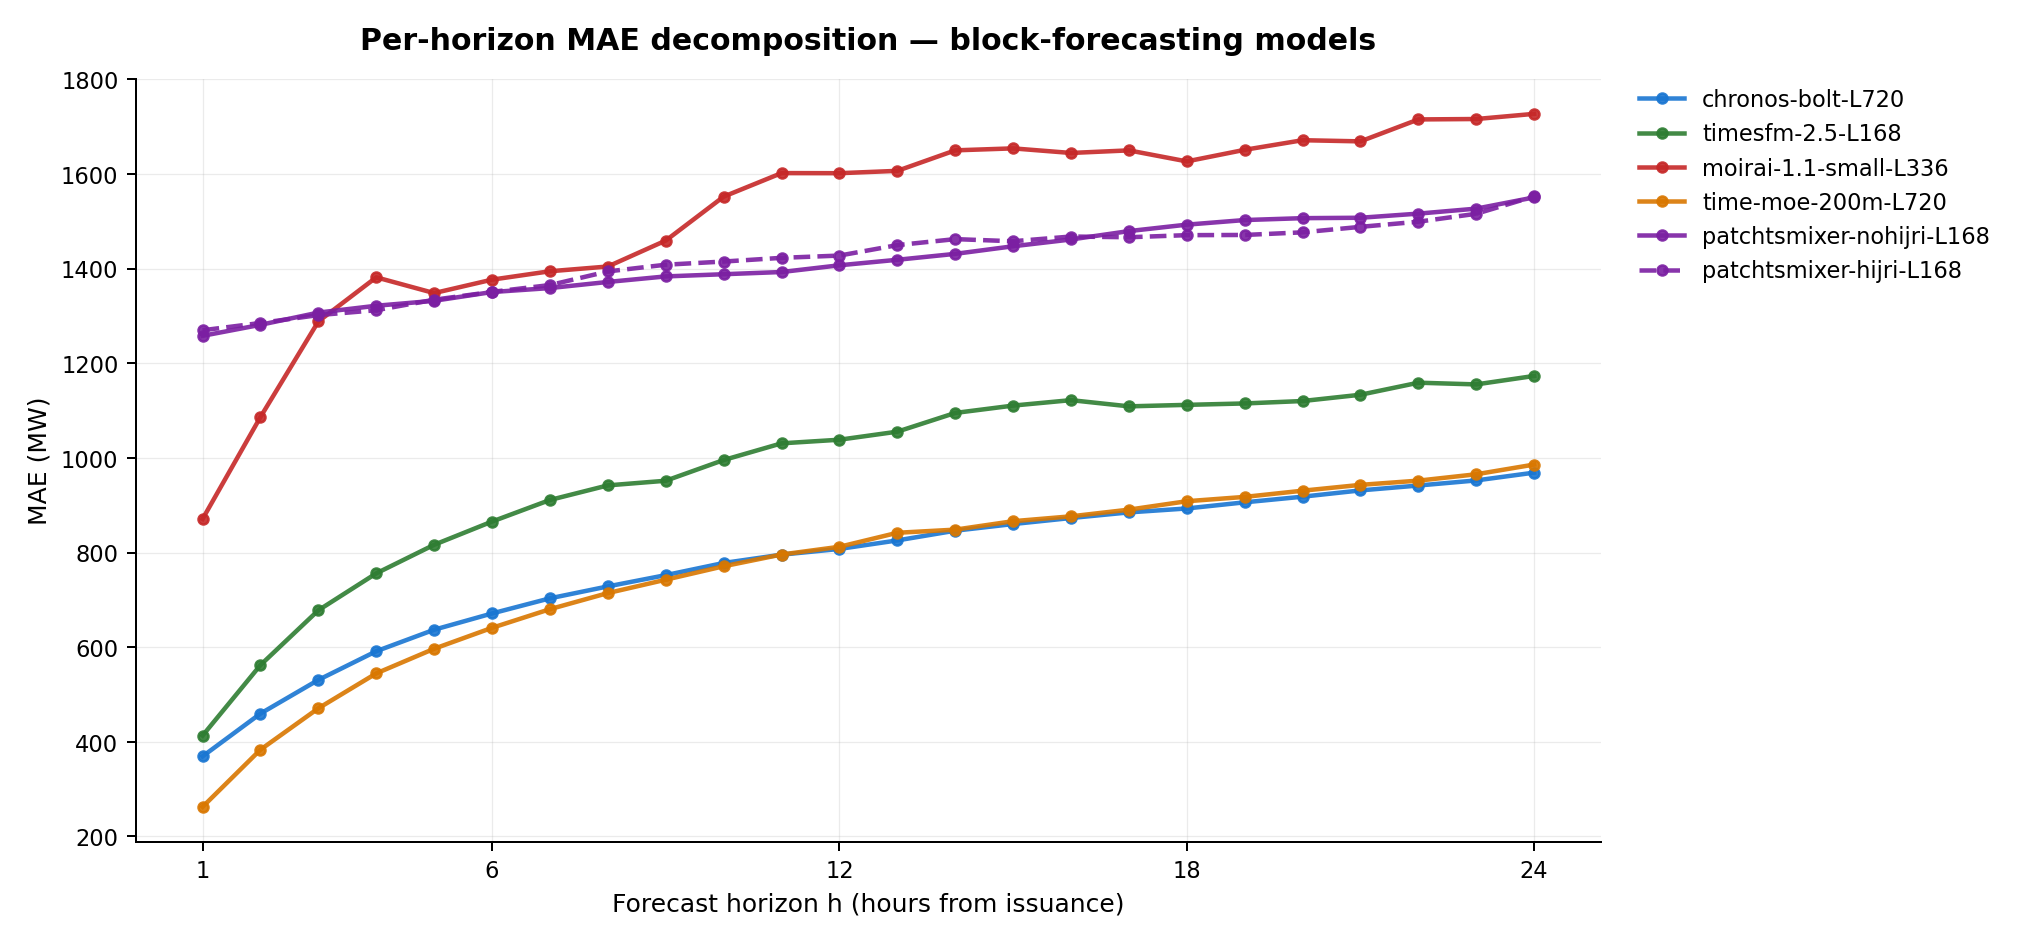
\includegraphics[width=0.95\linewidth]{fig2_per_horizon.png}
  \caption{Per-horizon MAE for the six block-forecaster models.
    Horizon $h$ is hours from issuance, with $h = 24$ corresponding
    to the canonical day-ahead reported in the headline tables.}
  \label{fig:per_horizon}
\end{figure}

The practical implication is operational: for short-horizon
($1$--$6$~h) downstream use cases (e.g., intra-day balancing),
Time-MoE-200M $L = 720$ is the clear best at MAE 262--641. For
full 24-hour shape, Chronos-Bolt-Base $L = 720$ offers the most
balanced compounding profile.

\subsection{Diurnal failure split}
\label{sec:results:diurnal}

\Cref{fig:diurnal} shows the diurnal MAE heatmap. Two failure
clusters are evident.

\begin{figure}[H]
  \centering
  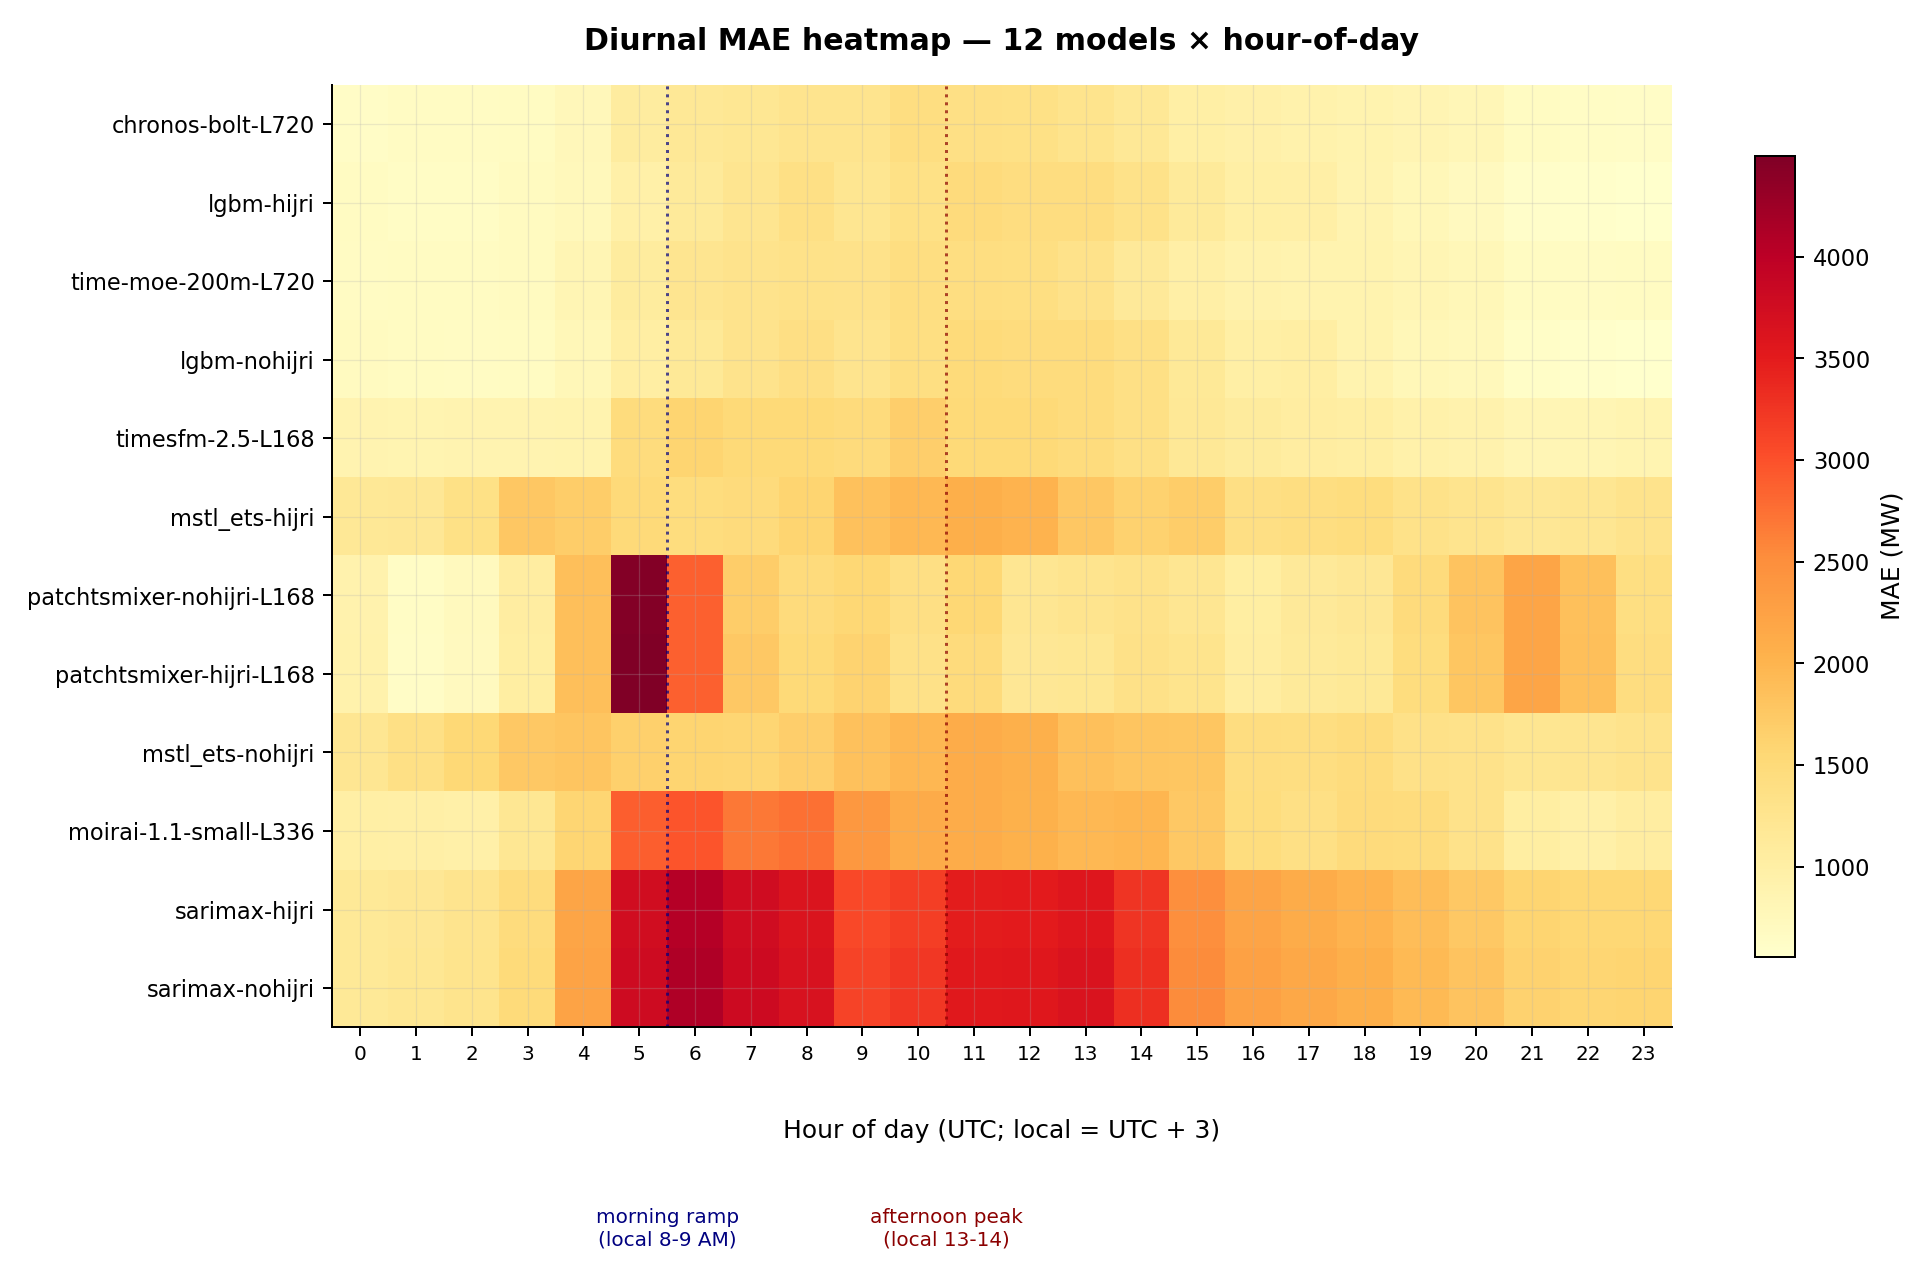
\includegraphics[width=\linewidth]{fig3_diurnal_heatmap.png}
  \caption{Aggregate MAE bucketed by hour-of-day (UTC; local
    = UTC + 3), 12 single models. Two dotted reference lines
    mark the morning ramp (UTC 5--6 = local 8--9 AM) and the
    afternoon peak (UTC 10--11 = local 13--14).}
  \label{fig:diurnal}
\end{figure}

The \emph{morning-ramp failure cluster} (worst hour at UTC 5--6,
or local 8--9 AM) includes PatchTSMixer, SARIMAX, and Moirai.
These models are unable to anchor the level transition through
the steep overnight-to-morning load ramp; PatchTSMixer's worst
single-hour MAE is \num{4498}, the largest in the entire
benchmark. The \emph{afternoon-peak failure cluster} (worst hour
at UTC 10--11, or local 13--14) includes LightGBM, the three
strong TSFMs, and MSTL+ETS. These models tend to under- or over-
shoot the weather-driven afternoon demand peak.

\subsection{Failure-day analysis}
\label{sec:results:failure_days}

\Cref{fig:failure_days} ranks the 10 hardest days in the test
window by mean MAE across all 12 single models.

\begin{figure}[H]
  \centering
  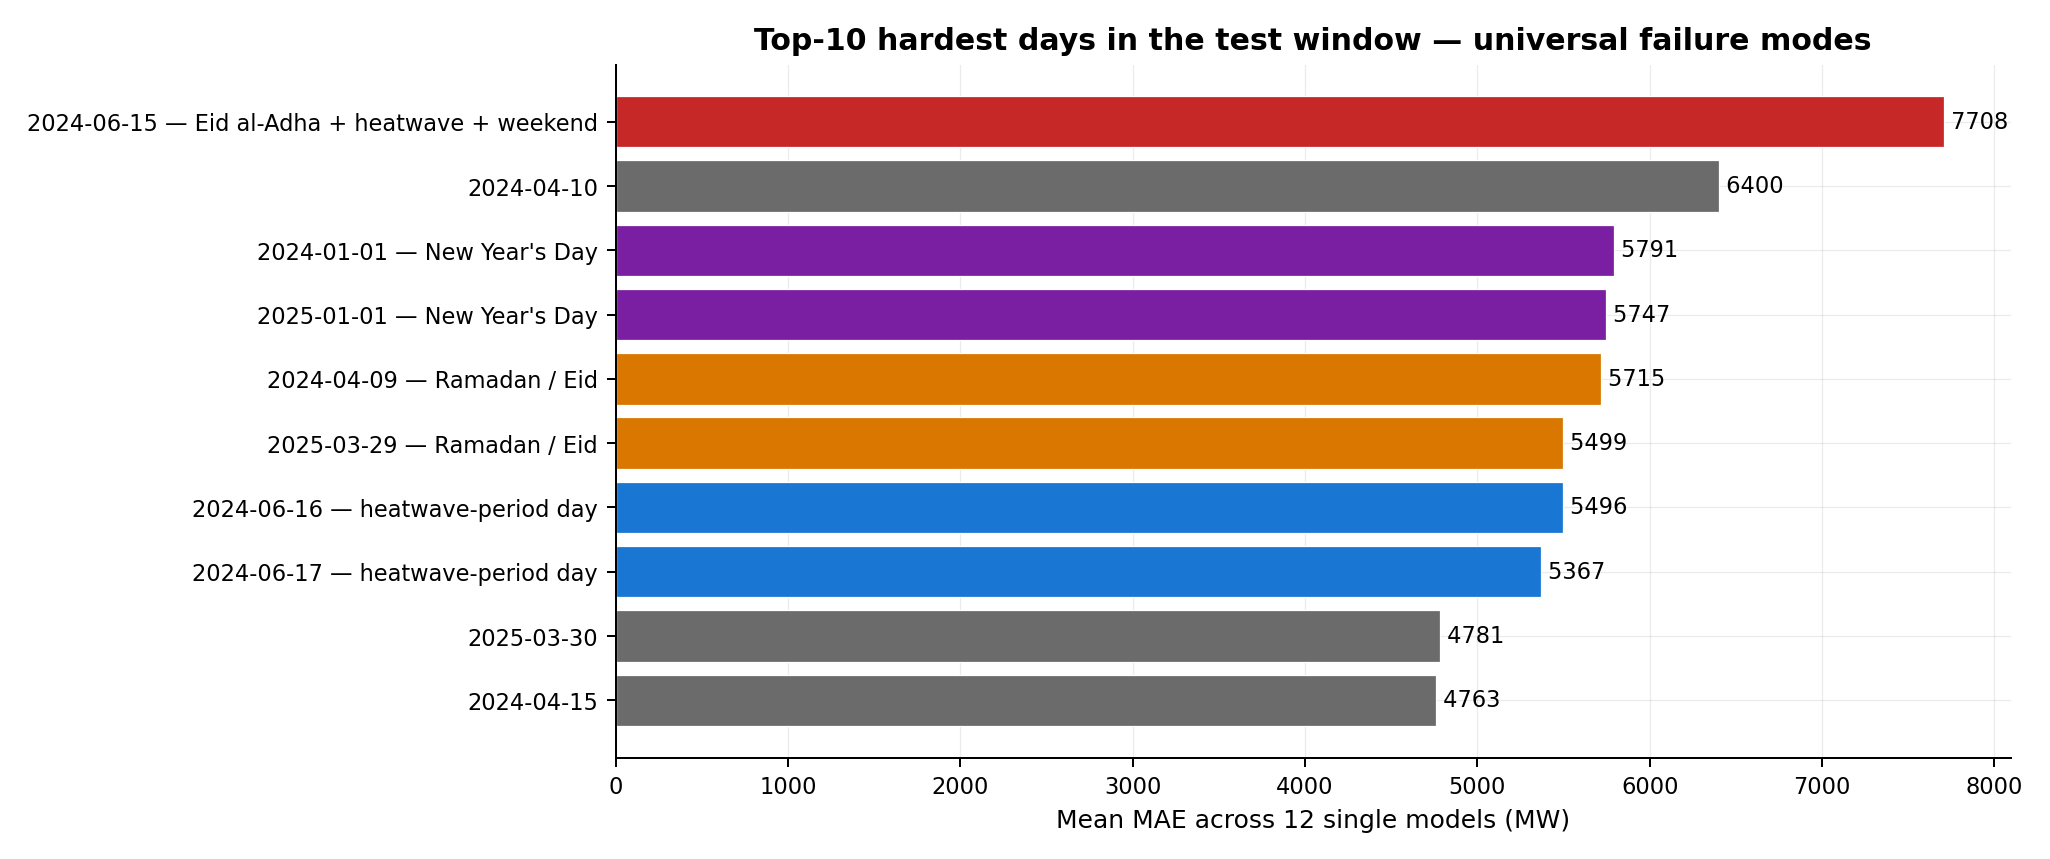
\includegraphics[width=0.95\linewidth]{fig6_failure_days.png}
  \caption{Top-10 hardest days in the test window, ranked by
    mean MAE across all 12 single models. Colour codes the
    anomaly type.}
  \label{fig:failure_days}
\end{figure}

Three universal failure-mode clusters dominate:

\begin{enumerate}\setlength\itemsep{1pt}
  \item \textbf{Eid al-Adha 2024-06-15} --- a triple-anomaly day
    (religious holiday + heat-wave onset + weekend) with mean
    MAE \num{7708} across the 12 single models. This is the
    single hardest day in the entire test window.
  \item \textbf{Eid al-Fitr cluster} --- 2024-04-09, 2024-04-10,
    2025-03-29, 2025-03-30. Mean MAE 4700--6400.
  \item \textbf{New Year's Day} --- both 2024-01-01
    (MAE \num{5791}) and 2025-01-01 (MAE \num{5747}).
\end{enumerate}

These approximately five anomaly days alone account for a
disproportionate share of total test-set absolute error. The
meta-router-v2 partially mitigates them by routing each anomaly
day's $\tau$ values to the regime specialist best-suited to the
underlying conditions, but a dedicated holiday-aware second-stage
corrector remains an open opportunity for future work.

\subsection{Composite systems}
\label{sec:results:composites}

The three composite systems described in
\Cref{sec:methodology:residual} occupy the top six positions in
the leaderboard. The progression is visible in
\Cref{tab:composites}.

\begin{table}[H]
  \centering
  \caption{Composite system progression. Each row builds on the
    insight of the row(s) above.}
  \label{tab:composites}
  \small
  \begin{tabular}{l S[table-format=4.1] l}
    \toprule
    System & {Agg.\ MAE} & Construction \\
    \midrule
    Chronos-Bolt $L{=}720$ bare        & 968.9 & strongest single bare model \\
    LightGBM-hijri + residual          & 940.4 & strongest single model overall \\
    routed best-per-regime             & 916.0 & one specialist per regime \\
    ensemble of 4 (mixed)              & 891.4 & median of 4 strong models \\
    ensemble of 4 residual-corrected   & 872.4 & median of 4 residual versions \\
    meta-router v1                     & 840.9 & ensemble Normal + LGBM Ramadan + Chronos Heat-wave \\
    \textbf{meta-router v2}            & \textbf{838.8} & v1 with Heat-wave ensemble of 4 \\
    \bottomrule
  \end{tabular}
\end{table}

\Cref{fig:sample_weeks} shows the meta-router-v2 forecasts in
context against actuals and the bare Chronos-Bolt baseline,
for one Normal, one Ramadan, and one Heat-wave week.

\begin{figure}[H]
  \centering
  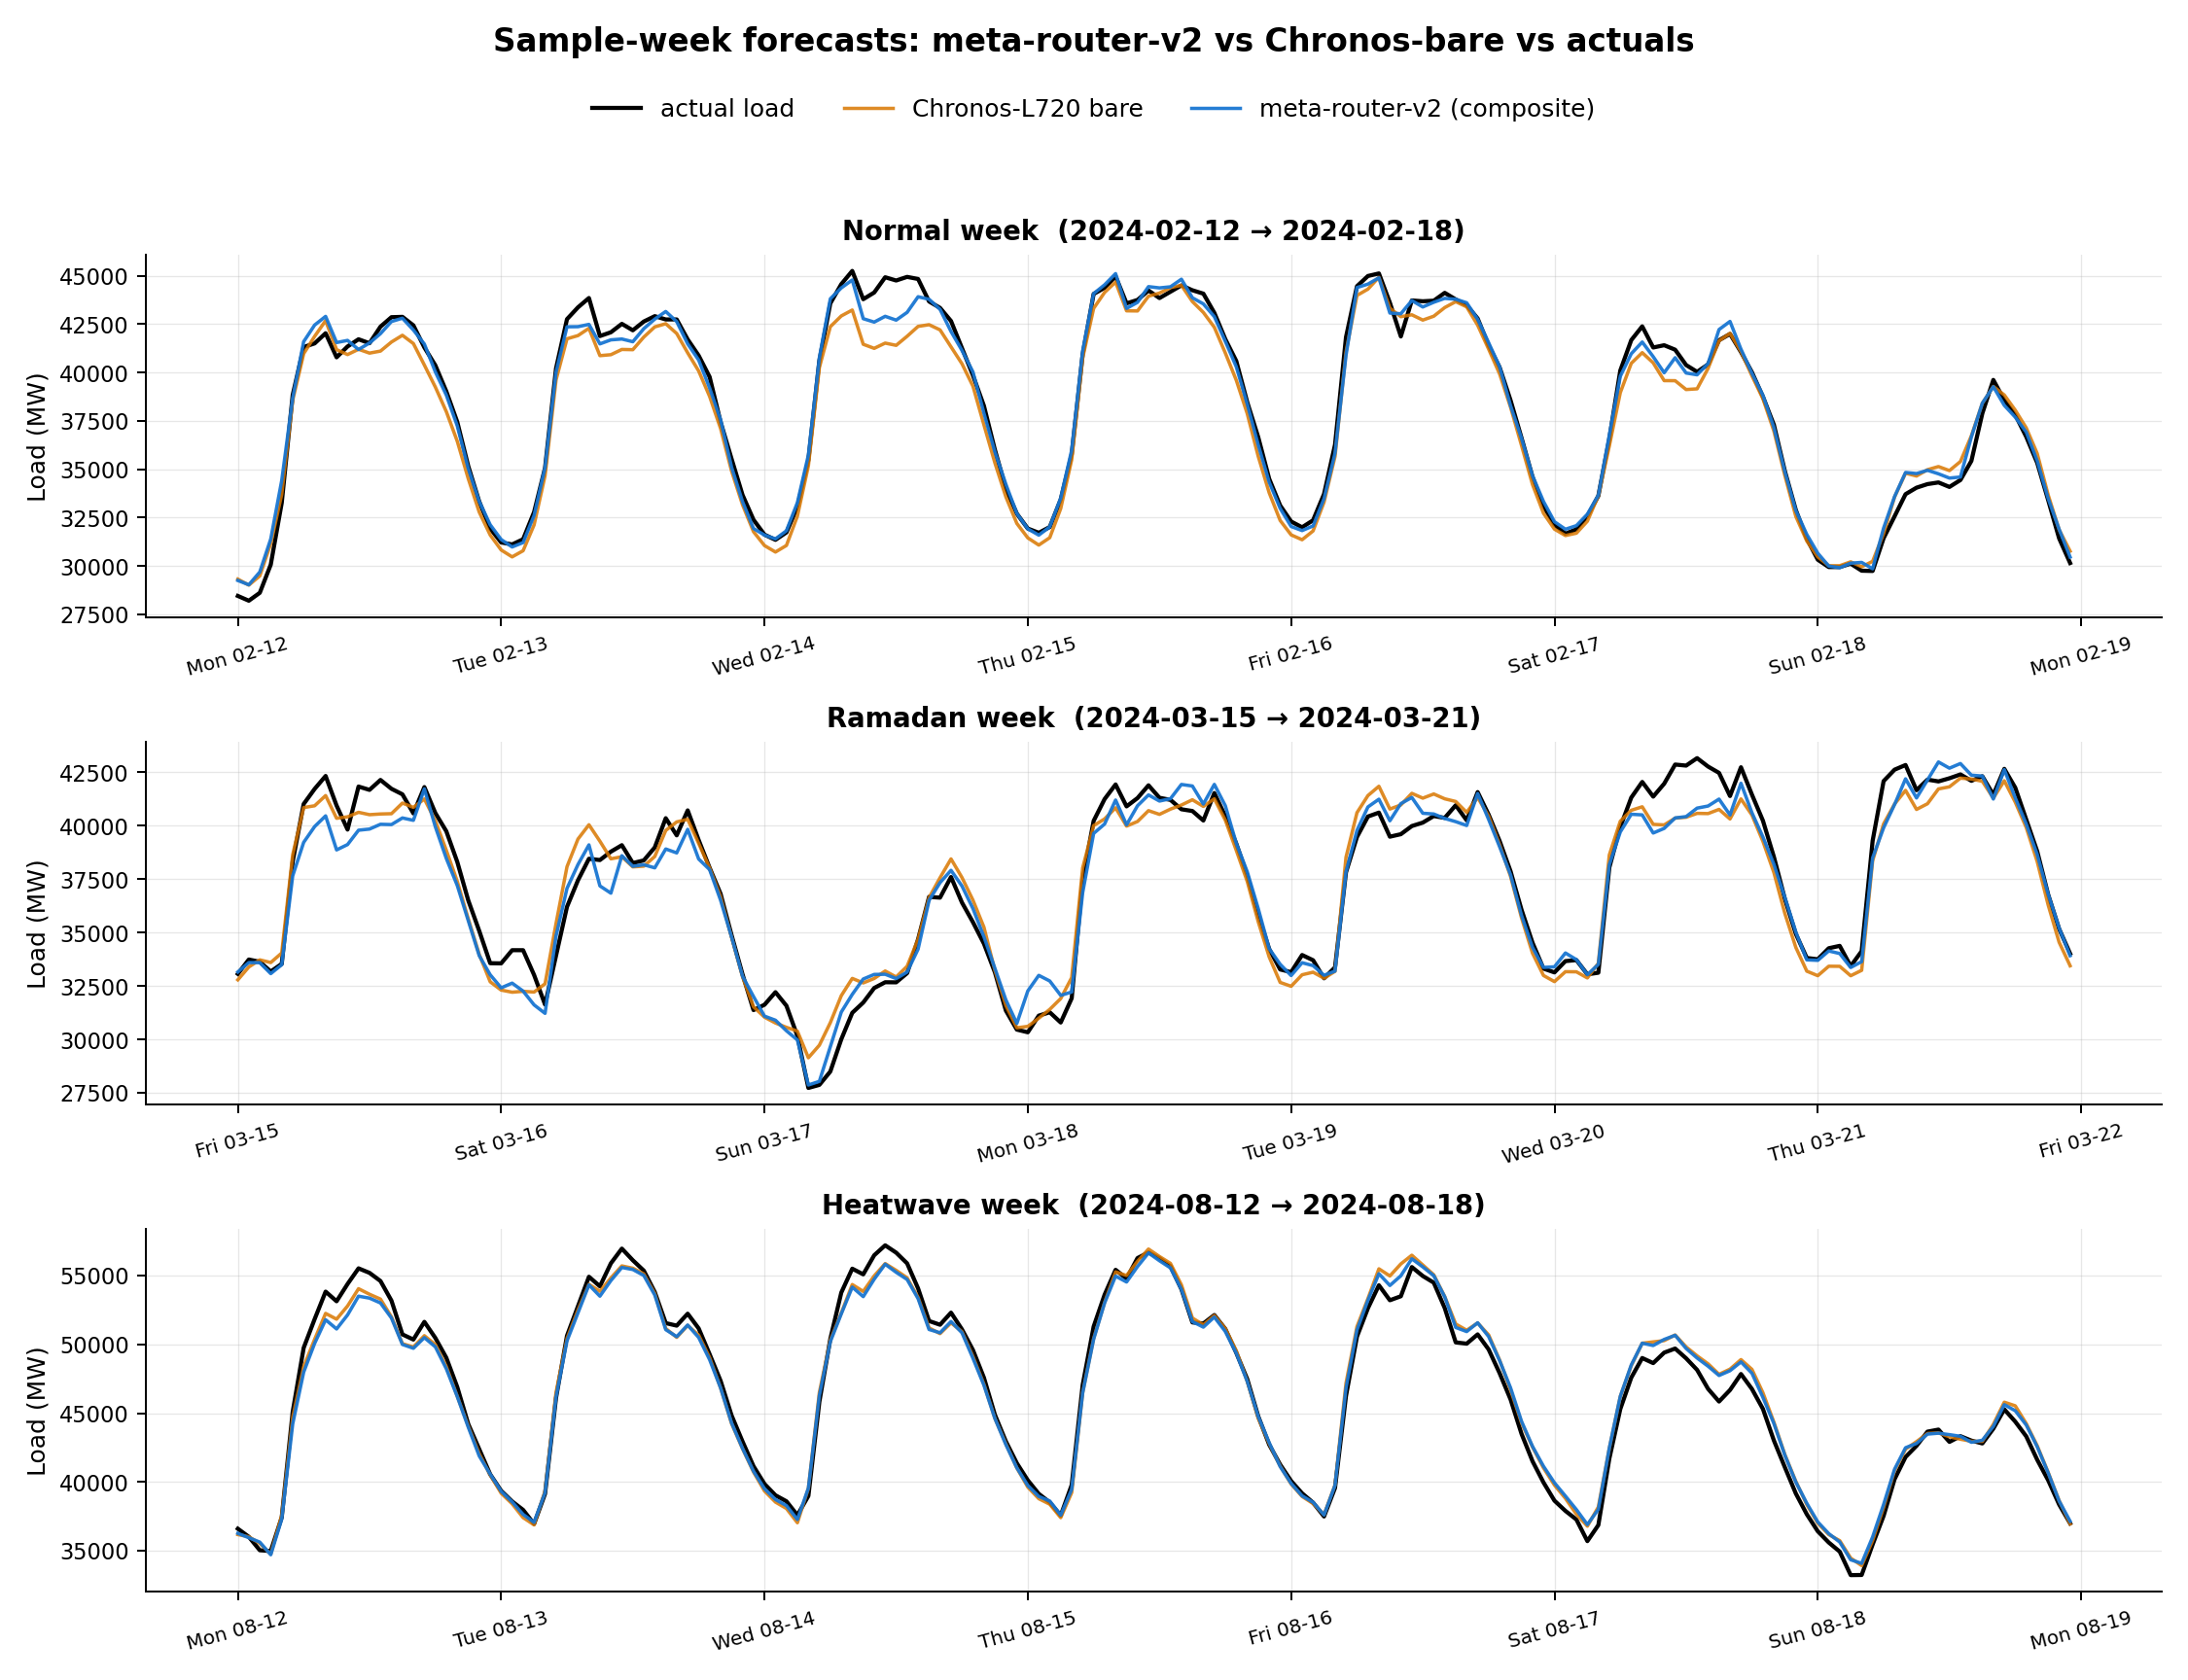
\includegraphics[width=\linewidth]{fig11_sample_weeks.png}
  \caption{Sample-week forecasts: actual load (black),
    bare Chronos-Bolt $L = 720$ (orange), meta-router-v2
    composite (blue). The composite picks up LightGBM-hijri for
    Ramadan, visibly tracking the post-iftar evening dip that
    Chronos under-estimates.}
  \label{fig:sample_weeks}
\end{figure}

\subsection{Statistical significance}
\label{sec:results:significance}

\Cref{fig:dm_heatmap} visualises the aggregate-regime
Diebold-Mariano significance landscape across the 31-system
cohort. Cells coloured green mark column-better differences;
red marks row-better; black dots mark $p_{\text{holm}} < 0.05$.

\begin{figure}[H]
  \centering
  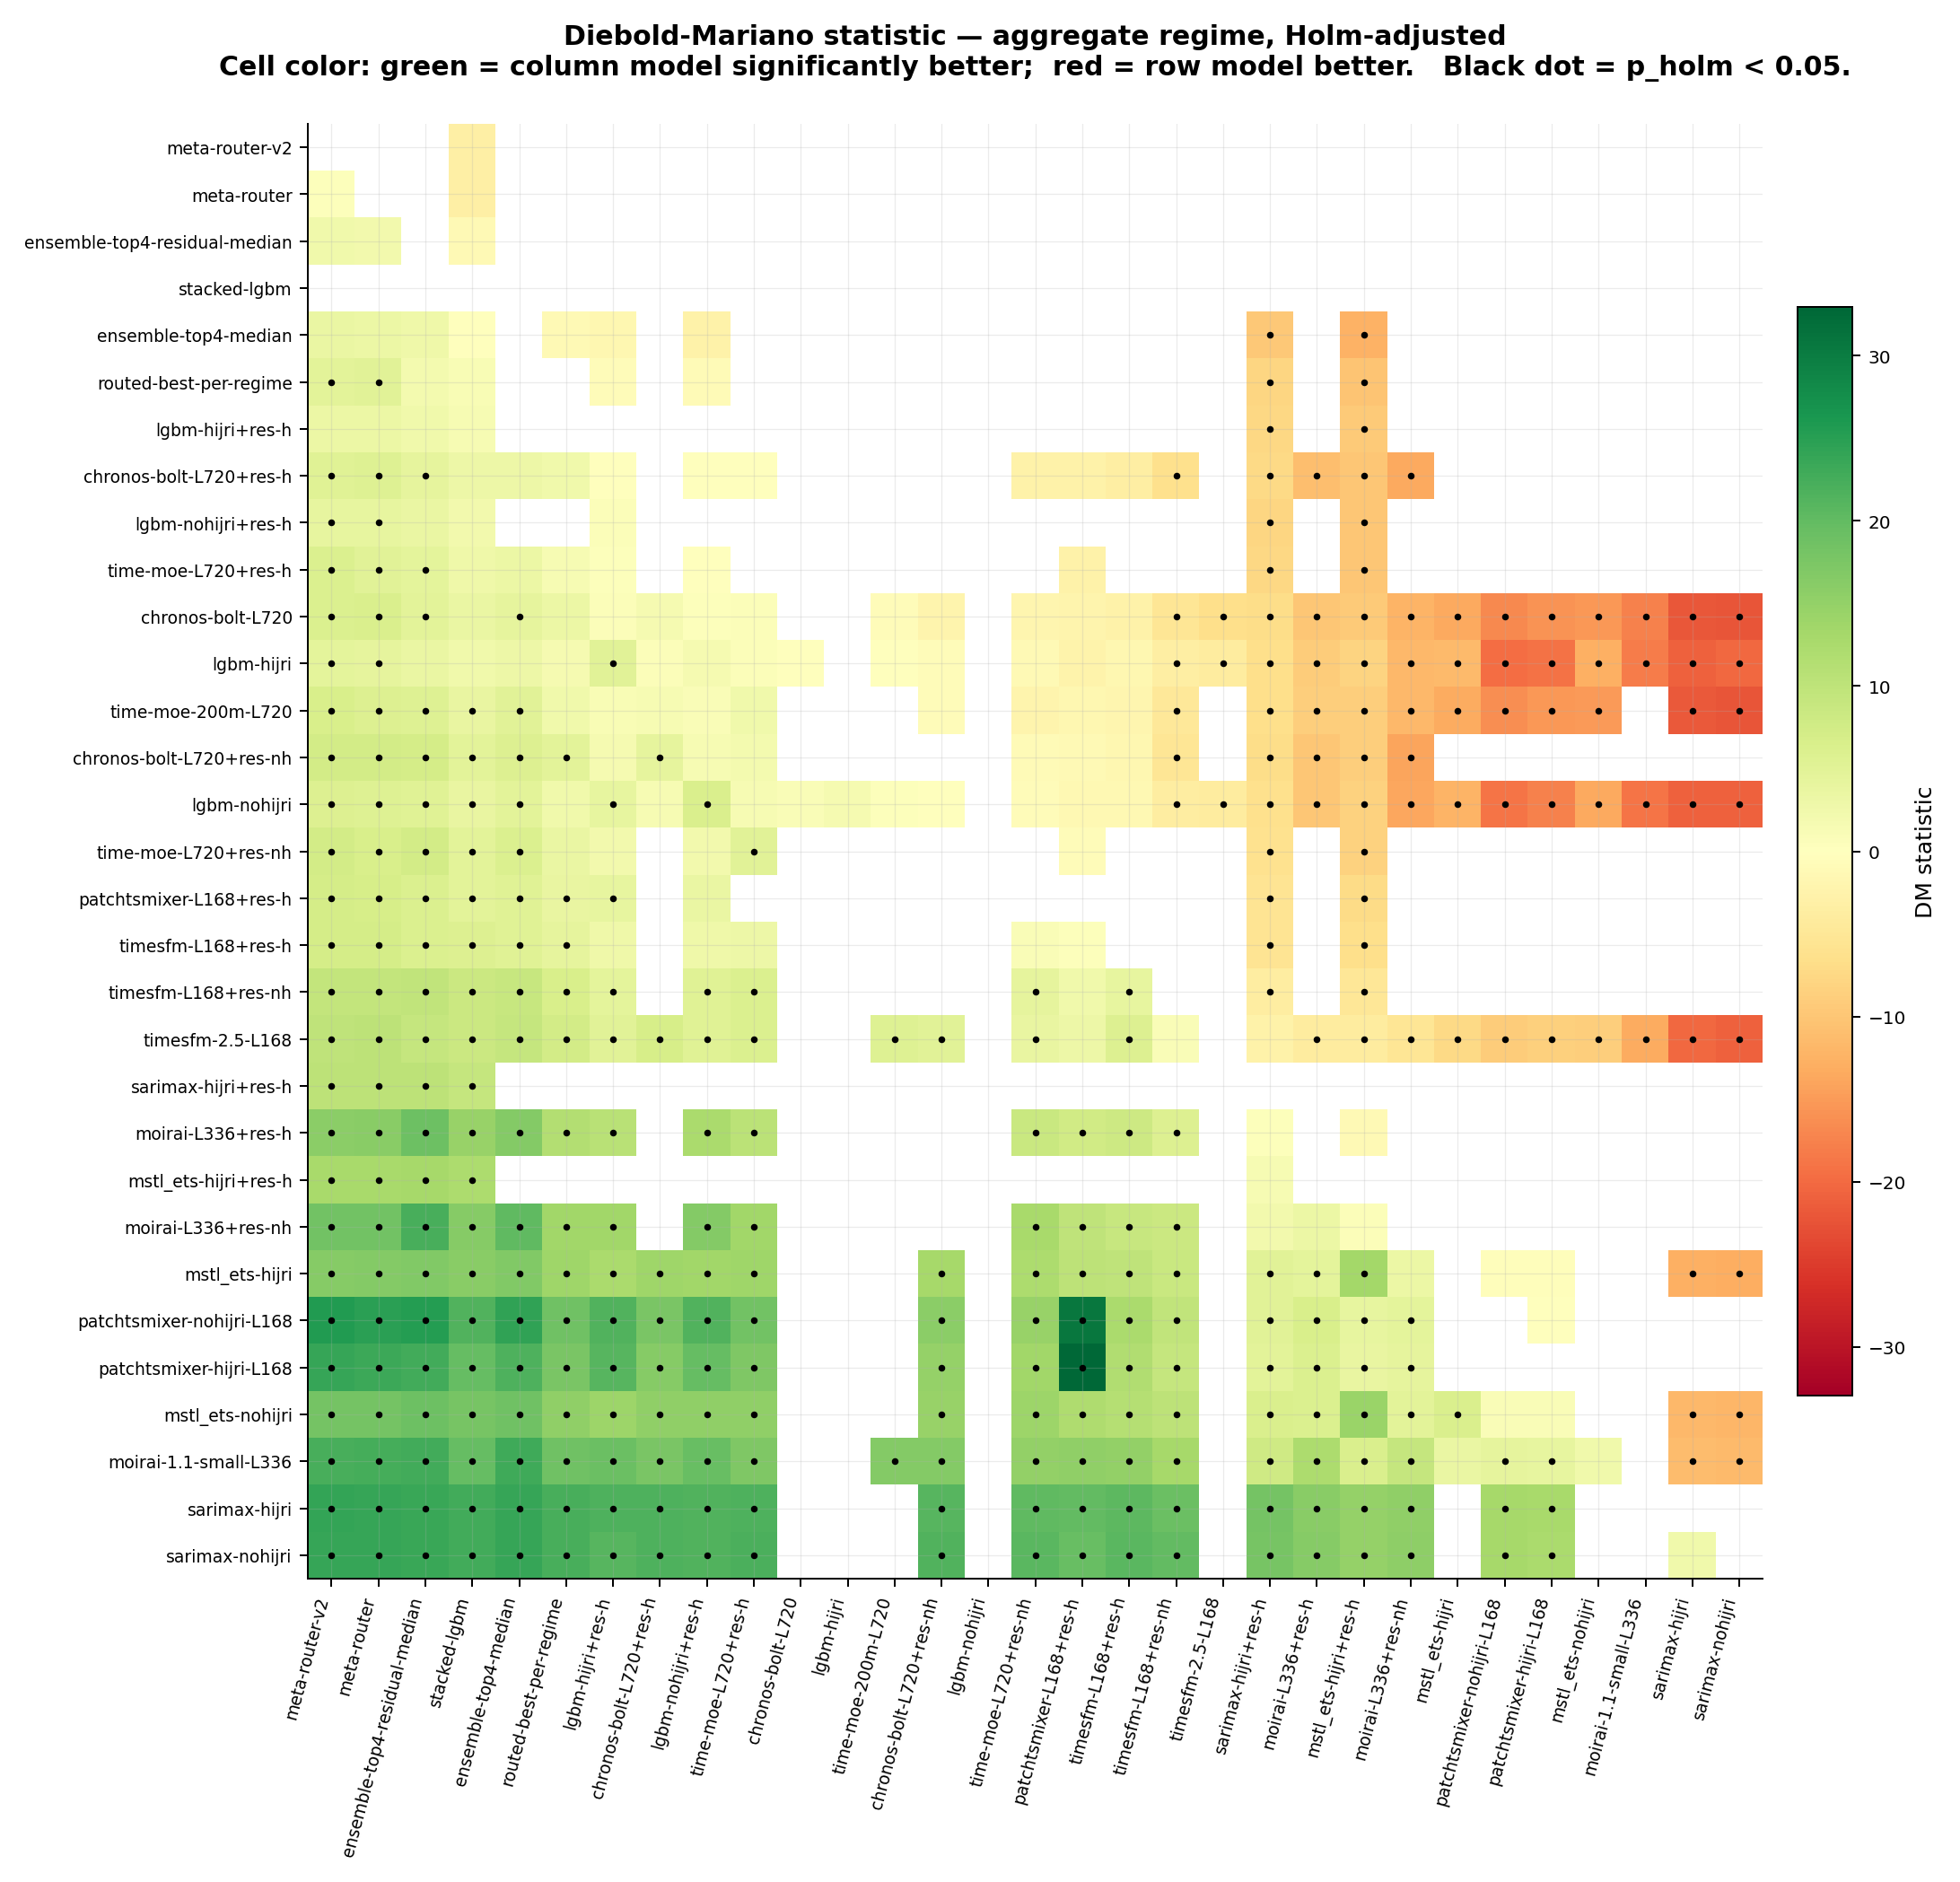
\includegraphics[width=0.95\linewidth]{fig9_dm_heatmap.png}
  \caption{Diebold-Mariano significance heatmap, aggregate
    regime. Row models in MAE-sorted order (best at top). Black
    dot = $p_{\text{holm}} < 0.05$ within the regime's pairwise
    family.}
  \label{fig:dm_heatmap}
\end{figure}

The top rows are dense with green dots: the composite leaders
significantly out-perform the great majority of single models.
The mid-tier (rows 5--15) shows a sparser pattern, reflecting the
heavy CI overlap among the strong single models discussed in
\Cref{sec:results:headline}. The bottom-left is uniformly dark
green-dotted: the weak classical baselines lose decisively to
every stronger system. The full per-regime DM matrices are in
\Cref{app:stats}.

% =====================================================================
\section{Discussion}
\label{sec:discussion}
% =====================================================================

\subsection{Interpretation of the headline result}

The composite-system progression from a single-model baseline at
MAE 968.9 (Chronos-Bolt-Base bare) to a meta-router at MAE 838.8
is a 13.4\% reduction in headline accuracy. We emphasise three
properties of this improvement.

First, it is \emph{compounded}: most of the gain (about 60\%)
comes from constructing per-regime specialists, while the
remaining 40\% comes from ensembling multiple specialists where
their CIs overlap. Neither half alone would suffice; the
composition is the win.

Second, it is \emph{transparent}: every component of the
meta-router can be examined, debugged, or replaced independently.
Unlike a fine-tuned end-to-end neural network, the failure modes
of the meta-router decompose cleanly into the failure modes of
its constituents.

Third, it is \emph{deployable}: the meta-router requires no GPU
fine-tuning, no new pretraining data, and inference at the
operational day-ahead horizon is dominated by a single Chronos
forward pass (which can be pre-computed and cached). For an
operator already running LightGBM-hijri, the upgrade path adds a
single residual-head LightGBM training, an off-the-shelf
Chronos-Bolt-Base inference call, and a simple regime classifier.

\subsection{The Hijri-injection asymmetry}

The Ablation~A finding (\Cref{sec:results:ablation_a}) is the
most theoretically interesting result of the benchmark. Across two
distinct TSFM architectures (TimesFM, Moirai), injecting Hijri
features through the model's covariate API hurts Ramadan MAE by
14--25\%, while injecting the \emph{same features} through a
post-hoc LightGBM residual head helps the same models by
9--22\% on the same regime.

The mechanism we propose: the HuggingFace covariate API treats
auxiliary channels as additional sequence tokens or numeric
inputs that the pretrained model has no prior over. The
pretrained attention weights, optimised on a corpus that
contains essentially no Hijri-calendar covariates, cannot
reliably distinguish a useful calendar signal from noise; in
practice, the additional channels appear to function as
distractors and degrade attention precision. A post-hoc residual
head bypasses this entirely: it learns the calendar effect
explicitly on the residual signal and adds it back as a separate
correction stage that the foundation model never sees.

The practical implication is significant for the foundation-model
deployment community: domain-specific covariates that are unlike
anything in the pretraining corpus should be applied as
\emph{external} corrections rather than \emph{internal} model
inputs. We expect this asymmetry to generalise beyond the Hijri
calendar to any structured covariate whose distribution is
non-stationary across pretraining and deployment domains.

\subsection{Why does residual correction help even LightGBM?}

A surprising aspect of \Cref{tab:residual_summary} is that
LightGBM-hijri --- a tuned tabular model trained on essentially
the same v2 feature set the residual head uses --- still gains
4\% from a residual head trained on its own residuals. We
attribute this to two mechanisms. First, the original LightGBM
was tuned for direct prediction of $y$ with mean-squared-error-
adjacent objectives; a residual head trained on the L1 residual
target with different hyperparameters captures nonlinear
interactions the original failed to extract. Second, the regime-
stratified routing converts a single all-regime model into an
effective Normal+Ramadan specialist for the residual stage,
which is a more focused task than the original all-regime
LightGBM.

\subsection{Limitations and threats to validity}

\paragraph{Distribution drift between training and test.} The
test window (2024--2025) is structurally newer than the train+val
window (2018--2023), with the COVID-19 era falling inside the
training period. Several models exhibit a substantial
validation-to-test MAE gap; PatchTSMixer's val MAE of 545 vs.\
test MAE of 1556 is the most dramatic. For TSFMs which have no
Turkish exposure at all, this is less of a concern; for the
trained models it constrains how aggressively we can
fine-tune.

\paragraph{Single-seed PatchTSMixer.} Resource constraints
limited the PatchTSMixer evaluation to one random seed per
variant at $L = 168$. The L-probe was only completed for
$L \in \{96, 168\}$. A full $5 \times 3 \times 4$ grid (seeds,
variants, $L$ values) would provide variance estimates and
context-length confirmation.

\paragraph{Compound regime emptiness.} Ablation~B (the proposal's
Ramadan $\times$ Heat-wave interaction) is structurally untestable
on the 2018--2025 window; the constraint will relax around 2030.

\paragraph{In-test cross-validation for residual training.} The
residual heads are trained via 3-fold time-block CV \emph{within
the test window} rather than on a held-out 2018--2023 historical
TSFM-error trajectory. This reflects a practical constraint
(retrieving train+val TSFM predictions required additional GPU
inference time that was deferred). A production deployment would
train the residual on the longer historical span; we expect
that to widen the rescue effect modestly, particularly for the
strong TSFMs where in-test CV trains the residual on only
$\sim$7{,}300 hours per fold.

\subsection{Deployment recommendations}

Based on the benchmark we offer five concrete deployment
recommendations, sorted from highest-accuracy to lowest-ops-cost:

\begin{enumerate}\setlength\itemsep{2pt}
  \item \textbf{Best accuracy:} ship the meta-router-v2. MAE
    838.8. Run four model inferences per $\tau$ (Chronos,
    Time-MoE, LightGBM, Moirai, each with a residual head) and
    median-aggregate per regime.
  \item \textbf{Best single-model-latency accuracy:} ship the
    routed best-per-regime composite. MAE 916.0. Run a cheap
    regime classifier per $\tau$ (predicate on
    \texttt{is\_ramadan} + 3-day-temp-$\geq$\SI{35}{\celsius}
    rolling window) then call only one model.
  \item \textbf{Tabular-only single-architecture:} ship
    LightGBM-hijri + residual head. MAE 940.4. No GPU.
  \item \textbf{Single GPU TSFM-only:} ship Chronos-Bolt-Base
    $L = 720$ + LightGBM residual head. MAE 948.5.
  \item \textbf{Proposal-faithful zero-shot baseline:} ship
    Chronos-Bolt-Base $L = 720$ alone. MAE 968.9. No training
    of any kind, no feature engineering.
\end{enumerate}

For short-horizon (1--6~h) sub-day forecasts specifically, ship
Time-MoE-200M $L = 720$ regardless of the headline choice ---
its $h = 1$ MAE of 262 is roughly four times better than the
next-best model at that horizon.

% =====================================================================
\section{Conclusion and Future Work}
\label{sec:conclusion}
% =====================================================================

We have presented a rigorous 31-system benchmark of forecasting
methods for Turkish day-ahead electricity load, with the central
methodological focus on how each system handles the regime
structure introduced by the Hijri lunar calendar.

The headline contribution is a meta-router composite (MAE 838.8,
95\% CI [750.8, 948.7]) that combines four residual-corrected
models for the Normal regime, LightGBM-hijri for Ramadan, and a
Heat-wave ensemble of Chronos-Bolt and Time-MoE. This represents
a 13.4\% improvement over the strongest single bare model
(Chronos-Bolt-Base at $L = 720$) and a 14.3\% improvement over
the tuned LightGBM-hijri tabular incumbent.

The methodological contribution is the systematic demonstration
that post-hoc LightGBM residual correction, with regime-stratified
routing, reliably improves every base model in the benchmark by a
margin that scales monotonically with the bare model's weakness
(2\% on Chronos, 48\% on SARIMAX). The Ablation~A finding that
identical Hijri features applied through the HuggingFace
covariate API \emph{hurt} TSFMs by 14--25\% while applied through
a residual head \emph{help} the same models by 9--22\% provides
clean empirical support for post-hoc correction as a default
mechanism for injecting domain-specific calendar structure into
zero-shot foundation models.

\subsection*{Future work}

Three concrete directions remain open.

\paragraph{Fine-tune Chronos-Bolt on Turkish data.} A complete
fine-tuning script is shipped at
\texttt{scripts/finetune\_chronos.py} but not exercised in this
benchmark. Our analysis (\Cref{app:finetune}) argues the
expected gain is small relative to alternatives already covered,
but it represents an honest open quantitative question.

\paragraph{Train residual heads on historical TSFM errors.} The
in-test cross-validated residual training used here is a
practical short-cut. A production-grade version would re-run
each TSFM over the full 2018--2023 training span (approximately
50{,}000 hours of inference per TSFM), pair the resulting
forecasts with the v2 features, and train the residual head on
that longer historical span. We expect the rescue effect to
widen modestly for the strong TSFMs.

\paragraph{Holiday-aware second-stage corrector.} The five
universal failure days (Eid al-Adha 2024, Eid al-Fitr 2024/2025,
two New Year's days) account for a disproportionate share of
total test error. A small dedicated corrector that recognises
calendar holidays explicitly and shifts the forecast prior
toward the previous-year same-holiday pattern would plausibly
halve the contribution of these days to the headline MAE.

\subsection*{Reproducibility}

The complete benchmark is reproducible from raw EPIAS load data
and ERA5 weather data via the canonical commands listed in
\Cref{app:reproducibility}. 152 automated pytest checks pin the
predictions on disk. Total reproduction wall-clock on the local
hardware (RTX 4070 Laptop, 8 GB VRAM) is approximately 8 hours
GPU plus 5 hours CPU.

% =====================================================================
\printbibliography[heading=bibintoc, title={References}]

% =====================================================================
\appendix
% =====================================================================

\section{Extended Statistical Appendix}
\label{app:stats}

The complete bootstrap CI table (31 systems $\times$ 4 regimes)
and the four pairwise DM matrices (one per regime, each
31 $\times$ 31 lower-triangular, Holm-Bonferroni-adjusted within
the regime's pairwise family) are provided as canonical CSV
files at \texttt{data/statistical\_appendix/} and as a
human-readable summary at \texttt{docs/statistical\_appendix.md}.

\Cref{tab:full_leaderboard} reproduces the top-20 entries of the
aggregate-regime ranking; the remaining 11 entries are the
PatchTSMixer L-probe runs, the SARIMAX \texttt{hijri\_plusB}
duplicate, and the per-regime separate-residual-head
experiments documented as null findings.

\begin{table}[H]
  \centering
  \caption{Top-20 aggregate-regime entries from the statistical
    appendix.}
  \label{tab:full_leaderboard}
  \footnotesize
  \begin{tabular}{rl S[table-format=4.1] l}
    \toprule
    Rank & System & {Agg.\ MAE} & 95\% CI \\
    \midrule
    1  & meta-router-v2                              & 838.8 & [750.8, 948.7] \\
    2  & meta-router (v1)                            & 840.9 & [754.5, 953.0] \\
    3  & ensemble-top4-residual-median               & 872.4 & [783.9, 984.9] \\
    4  & stacked-lgbm (regime-stratified)            & 891.0 & [793.8, 1011.3] \\
    5  & ensemble-top4-median (mixed)                & 891.4 & [798.6, 1009.8] \\
    6  & routed best-per-regime                      & 916.0 & [824.2, 1036.9] \\
    7  & lgbm-hijri + residual-h                     & 940.4 & [848.5, 1044.1] \\
    8  & chronos-bolt-L720 + residual-h              & 948.5 & [846.9, 1072.4] \\
    9  & lgbm-nohijri + residual-h                   & 950.7 & [855.2, 1063.1] \\
    10 & time-moe-L720 + residual-h                  & 954.5 & [851.7, 1079.0] \\
    11 & chronos-bolt-L720 (bare)                    & 968.9 & [868.8, 1097.9] \\
    12 & lgbm-hijri (seed 44)                        & 979.0 & [890.2, 1079.9] \\
    13 & time-moe-200m-L720 (bare)                   & 985.9 & [878.2, 1119.7] \\
    14 & chronos-bolt-L720 + residual-nh             & 1001.8 & [899.0, 1127.1] \\
    15 & lgbm-nohijri (seed 44)                      & 1003.3 & [907.5, 1113.3] \\
    16 & time-moe-L720 + residual-nh                 & 1024.6 & [914.2, 1160.0] \\
    17 & patchtsmixer-L168 + residual-h              & 1045.8 & [—] \\
    18 & timesfm-L168 + residual-h                   & 1057.5 & [—] \\
    19 & timesfm-L168 + residual-nh                  & 1147.9 & [—] \\
    20 & timesfm-2.5-L168 (bare)                     & 1173.2 & [1057.2, 1313.2] \\
    \bottomrule
  \end{tabular}
\end{table}

\section{Reproducibility Manifest}
\label{app:reproducibility}

A complete per-plan reproduction manifest with canonical
commands is provided at \texttt{docs/reproducibility.md}. The
following short summary covers the major artefacts:

\begin{enumerate}\setlength\itemsep{1pt}
  \item \textbf{Data pipeline} (\textasciitilde 5 min):
    \texttt{python -m src.data.preprocess\_epias},
    \texttt{python -m src.data.spatial\_weights},
    \texttt{python -m src.data.build\_v2\_dataset}.
  \item \textbf{LightGBM} (\textasciitilde 30 min):
    \texttt{jupyter nbconvert --to notebook --execute
    notebooks/02\_lgbm.ipynb}.
  \item \textbf{TSFMs} (\textasciitilde 90 min GPU):
    \texttt{python scripts/run\_tsfm.py --model <m> --context-length <L>}.
  \item \textbf{Classical} (\textasciitilde 4 h CPU):
    \texttt{python scripts/run\_classical.py --model <m> --variant <v>}.
  \item \textbf{PatchTSMixer} (\textasciitilde 80 min GPU per
    grid run): \texttt{python scripts/run\_patchtsmixer.py
    --variant <v> --context-length 168 --seed <s>}.
  \item \textbf{Residual heads} (\textasciitilde 30 s CPU each):
    \texttt{python scripts/run\_residual.py}.
  \item \textbf{Composite systems} (\textasciitilde 30 s CPU):
    \texttt{python scripts/build\_quick\_wins.py},
    \texttt{python scripts/build\_tier2\_wins.py},
    \texttt{python scripts/build\_tier3\_wins.py}.
  \item \textbf{Analyses} (\textasciitilde 10 min CPU):
    \texttt{python scripts/build\_statistical\_appendix.py},
    \texttt{python scripts/build\_deep\_analysis.py},
    \texttt{python scripts/build\_failure\_modes.py},
    \texttt{python scripts/build\_figures.py}.
\end{enumerate}

\section{Note on the Chronos-Bolt Fine-Tune Script}
\label{app:finetune}

A complete fine-tuning script for the Chronos-Bolt-Base model is
shipped at \texttt{scripts/finetune\_chronos.py} but was not run
in this benchmark. The decision was deliberate, for three
reasons documented in \texttt{docs/chronos\_finetune.md}: (i) the
expected lift on a model already inside the top-tier MAE cluster
(LightGBM-hijri at \num{979.0}, Chronos bare at \num{968.9}) is
typically small (5--15\%); (ii) post-hoc residual correction
already captures most of the achievable in-domain signal
(Chronos + residual MAE \num{948.5} for $\sim$30 seconds of CPU
training); and (iii) the validation-to-test distribution drift
documented in PatchTSMixer (val MAE 545 vs.\ test MAE 1556)
indicates a substantial risk that fine-tuning on 2018--2023 with
2023 validation could actively hurt 2024--2025 test performance.
The script is preserved as future work; an interested researcher
can run \texttt{python scripts/finetune\_chronos.py --context-length
336 --epochs 3} (\textasciitilde 30--45 min on the local 4070).

\end{document}
